\documentclass{book}
\tolerance 500%
\emergencystretch 1em\relax
\hfuzz .2pt\relax
\usepackage{latexml}
\usepackage{../sty/latexmlman}
\usepackage{times}
\usepackage{makeidx}
\usepackage{listings}
\usepackage{tocbibind}
\usepackage{wrapfig}
% Should the additional keywords be indexed?
\lstdefinestyle{shell}{language=bash,escapechar=@,basicstyle=\ttfamily\iflatexml\else\small\fi,%
   morekeywords={latexml,latexmlpost,latexmlmath},
   moredelim=[is][\itshape]{\%}{\%}}
\lstdefinestyle{latexml}{basicstyle=\ttfamily\iflatexml\else\small\fi,language=Perl,%
   morekeywords={CC_ESCAPE,CC_BEGIN,CC_END,CC_MATH,CC_ALIGN,CC_EOL,CC_PARAM,CC_SUPER,%
     CC_SUB,CC_IGNORE,CC_SPACE,CC_LETTER,CC_OTHER,CC_ACTIVE,CC_COMMENT,CC_INVALID,CC_CS,CC_NOTEXPANDED,%
     T_BEGIN,T_END,T_MATH,T_ALIGN,T_PARAM,T_SUB,T_SUPER,T_SPACE,T_LETTER,T_OTHER,T_ACTIVE,T_COMMENT,T_CS,T_CR,%
     Token,Tokens,Tokenize,TokenizeInternal,Explode,UnTeX,StartSemiverbatim,EndSemiverbatim,%
     Number,Float,Dimension,MuDimension,Glue,MuGlue,Pair,PairList,%
     NoteProgress,NoteBegin,NoteEnd,Fatal,Error,Warn,Info,%
     Stringify,ToString,Equals,%
     DefExpandable,DefMacro,DefMacroI,DefPrimitive,DefPrimitiveI,DefRegister,DefRegisterI,%
     DefConstructor,DefConstructorI,dualize_arglist,
     DefMath,DefMathI,DefEnvironment,DefEnvironmentI,convertLaTeXArgs,%
     RequirePackage,LoadClass,FindFile,DeclareOption,PassOptions,ProcessOptions,ExecuteOptions,AddToMacro,%
     NewCounter,CounterValue,StepCounter,RefStepCounter,RefStepID,ResetCounter,GenerateID,%
     Tag,DocType,RelaxNGSchema,RegisterNamespace,%
     DefRewrite,DefMathRewrite,DefLigature,DefMathLigature,%
     Expand,Invocation,Digest,RawTeX,Let,%
     ReadParameters,DefParameterType,DefColumnType,%
     LookupValue,AssignValue,PushValue,PopValue,UnshiftValue,ShiftValue,LookupCatcode,AssignCatcode,%
     LookupMeaning,LookupDefinition,InstallDefinition,%
     CleanLabel,CleanIndexKey,CleanBibKey,CleanURL,UTF,roman,Roman,%
     MergeFont,%
     CheckOptions},
}
\lstdefinestyle{xml}{basicstyle=\small\sffamily,language=xml,escapechar=@}%
\lstdefinestyle{inlinelatexml}{style=latexml,moredelim=[is][\itshape\small]{\%}{\%},escapechar=@}
\newcommand{\shellcode}{\lstinline[style=shell]}
\newcommand{\ltxcode}{\lstinline[style=inlinelatexml]}
\newcommand{\perlcode}{\lstinline[style=Perl]}
\newcommand{\xmlcode}{\lstinline[style=xml]}

\input{release.tex}
\makeindex

\title{\LaTeXML\ \emph{The Manual}}
\subtitle{A \LaTeX\ to \XML/\HTML/\MathML\ Converter;\\ Version \emph{\CurrentVersion}}
\author{Bruce R.~Miller}
\lxKeywords{LaTeXML, LaTeX to XML, LaTeX to HTML, LaTeX to MathML, LaTeX to ePub, converter}
%============================================================
\begin{lxNavbar}
\lxRef{top}{\includegraphics{../graphics/latexml}}\\
\includegraphics{../graphics/mascot}\\
\lxContextTOC
\end{lxNavbar}
%============================================================
\begin{document}\label{top}
\frontmatter
\iflatexml
\maketitle
\else
\begin{titlepage}
\parindent=0em
\makeatletter
\null\vfil
\hbox to \textwidth{%
  \hfill
  \hbox to 0.5in {
  \includegraphics{../graphics/mascot.png} }
%  \kern -2in
%  \hskip -1.5in
 \vbox{
   \null
    \centering
    {\LARGE \@title \par}%
    \vskip 1.0em%
    {\large \@subtitle \par}%
    \vskip 3em%
    {\large \@author \par}
    \vskip 1.5em%
    {\large \@date \par}%       % Set date in \large size.
    \vskip 3em%
   \null
   }
  \hfill
}
\par\vfil\null
\makeatother
\end{titlepage}
\fi
\tableofcontents
\listoffigures
\mainmatter
%%%======================================================================
% \part{Basics}
%%%======================================================================
\chapter{Introduction}\label{intro}
\begin{advanced}
\paragraph{Note:}\label{intro.note}
Some of the more detailed portions of this manual have
not kept uptodate with the evolution of the code and style of \LaTeXML,
but rather than delay release, we'll improve the documentation in a later update.
\end{advanced}

For many, \LaTeX\ is the preferred format for document authoring, particularly those
involving significant mathematical content and where quality typesetting is desired.
On the other hand, content-oriented \XML\ is an extremely useful representation for documents,
allowing them to be used, and reused, for a variety of purposes, not least, 
presentation on the Web. Yet, the style and intent of \LaTeX\ markup, as compared to \XML\
markup, not to mention its programmability, presents difficulties in converting
documents from the former format to the latter.
Perhaps ironically, these difficulties can be particularly large for mathematical material, 
where there is a tendency for the markup to focus on appearance rather than meaning.

The choice of \LaTeX\ for authoring, and \XML\ for delivery were natural and uncontroversial
choices for the \URL[Digital Library of Mathematical Functions]{http://dlmf.nist.gov}.
Faced with the need to perform this conversion and the lack of suitable tools to perform it, 
the DLMF project proceeded to develop thier own tool, \LaTeXML, for this purpose.
%This document describes a \emph{preview} release of \LaTeXML.

\paragraph{Design Goals}\label{intro.goals} The idealistic goals of \LaTeXML\ are:
\begin{itemize}
\item Faithful emulation of \TeX's behaviour;
\item Easily extensible;
\item Lossless, preserving both semantic and presentation cues;
\item Use an abstract \LaTeX-like, extensible, document type;
\item Infer the semantics of mathematical content\\
    (\emph{Good} Presentation \MathML, eventually Content \MathML\ and \OpenMath).
\end{itemize}

As these goals are not entirely practical, even somewhat contradictory,
they are implicitly modified by \emph{as much as possible}.
Completely mimicing \TeX's, and \LaTeX's, behaviour would seem to require the
sneakiest modifications to \TeX, itself; redefining \LaTeX's internals does 
not really guarantee compatibility. ``Ease of use'' is, of course, in the eye of the beholder;
this manual is an attempt to make it easier!
More significantly, few documents are likely to have completely unambiguous
mathematics markup; human understanding of both the topic and the surrounding 
text is needed to properly interpret any particular fragment.
Thus, while we'll try to provide a ``turn-key'' solution that does the `Right Thing'
automatically, we expect that applications requiring high semantic content will require
document-specific declarations and tuning to achieve the desired result.
Towards this end, we provide a variety
of means to customize the processing and declare the author's intent.
At the same time, especially for new documents, we encourage a more logical, 
content-oriented markup style, over a purely presentation-oriented style.

\paragraph[Overview]{Overview of this Manual}\label{intro.overview}
Chapter \ref{usage} describes the usage of \LaTeXML, along with
common use cases and techniques.  Chapter \ref{architecture} describes
the system architecture in some detail. Strategies for customization
and implementation of new packages is described in Chapter \ref{customization}.
The special considerations for mathematics, including details of representation
and how to improve the conversion, are covered in Chapter \ref{math}.
Several specialized topics are covered in the remaining chapters.
An overview of outstanding issues and planned future improvements
are given in Chapter \ref{todo}.

Finally, the Appendices give detailed documentation the system components:
Appendix \ref{commands} describes the command-line programs provided by the system;
Appendix \ref{included.bindings} lists the \LaTeX\ style packages for which
we've provided \LaTeXML-specific bindings.
Appendix \ref{modules}
describes the various Perl modules, in groups, that comprise the system.
Appendix \ref{schema} describes the \XML\ schema used by \LaTeXML.
Appendix \ref{errorcodes} gives an overview of the warning and
error messages that \LaTeXML\ may generate.
Appendix \ref{cssclasses} describes the strategy and naming conventions
used for CSS styling of the resulting \HTML.

Using \LaTeXML, and programming for it, can be somewhat confusing as one is dealing with several
languages not normally combined, often within the same file,
--- Perl, \TeX\ and \XML\ (along with \XSLT, \HTML, \CSS),
plus the occasional shell programmming.
To help visually distinguish different contexts in this manual
we will put `programming' oriented material (Perl, \TeX) in a typewriter font,
\texttt{like this}; \XML\ material will be put in a sans-serif face
\textsf{like this}.

\vskip 1cm\relax
If you encounter difficulties, there is a support mailing list at
\URL[\texttt{latexml-project}]{http://lists.informatik.uni-erlangen.de/mailman/listinfo/latexml}.
Bugs and enhancement requests can be reported at
\URL[Github]{https://github.com/brucemiller/LaTeXML}.
If all else fails, please consult the source code, or the author.

\begin{advanced}
Danger! When you see this sign, be warned that the material presented is
somewhat advanced and may not make much sense until you have dabbled quite
a bit in \LaTeXML's internals.
Such advanced or `dangerous' material will be presented like this paragraph
to make it easier to skip over.
\end{advanced}

%%%======================================================================
\chapter{Using \LaTeXML}\label{usage}
The main commands provided by the \LaTeXML\ system are
\begin{description}
\item[\ltxcmd{latexml}] for converting \TeX\ and \BibTeX\ sources to \XML.
\item[\ltxcmd{latexmlpost}] for various postprocessing tasks including
conversion to \HTML, processing images, conversion to \MathML\ and so on.
\end{description}
\noindent The usage of these commands can be as simple as
\begin{lstlisting}[style=shell]
latexml doc.tex | latexmlpost --dest=doc.html -
\end{lstlisting}
\noindent to convert a single document into \textsc{HTML5} document,
 or as complicated as
\begin{lstlisting}[style=shell]
latexml --dest=1.xml ch1
latexml --dest=2.xml ch2
@ \hbox{}\hspace{1in}$\vdots$ @
latexml --dest=b.xml b
latexml --dest=B.bib.xml B.bib
latexmlpost --prescan --db=my.db --dest=1.html 1
latexmlpost --prescan --db=my.db --dest=2.html 2
@ \hbox{}\hspace{1in}$\vdots$ @
latexmlpost --prescan --db=my.db --dest=b.html b
latexmlpost --noscan --db=my.db  --dest=1.html 1
latexmlpost --noscan --db=my.db  --dest=2.html 2
@ \hbox{}\hspace{1in}$\vdots$ @
latexmlpost --noscan --db=my.db  --dest=b.html b
\end{lstlisting}
\noindent to convert a whole set of documents, including a bibliography,
into a complete interconnected site.

How best to use the commands depends, of course, on what you
are trying to achieve.  In the next section, we'll describe
the use of \ltxcmd{latexml}, which performs the conversion to \XML.
The following sections consider a sequence of
successively more complicated postprocessing situations,
using \ltxcmd{latexmlpost},
by which one or more \TeX\ sources can be converted into
one or more web documents or a complete site.

Additionally, there is a convenience command \ltxcmd{latexmlmath}
for converting individual formula into various formats.

%%%----------------------------------------------------------------------
\section[Conversion]{Basic \XML\ Conversion}\label{usage.conversion}\index{latexml!basic usage}
The command
\begin{lstlisting}[style=shell]
latexml {options} --destination=%doc%.xml %doc%
\end{lstlisting}
converts the \TeX\ document \texttt{doc.tex},
or standard input if \texttt{-} is used in place of the filename, to \XML.
It loads any required definition bindings (see below),
reads, tokenizes, expands and digests the document creating an \XML\ structure.
It then performs some document rewriting, parses the mathematical content
and writes the result, in this case, to \texttt{doc.xml};
if no \shellcode|--destination| is suppplied, it writes the result to standard output.
For details on the processing, see Chapter \ref{architecture},
and Chapter \ref{math} for more information about math parsing.

\paragraph{\BibTeX\ processing}\label{usage.conversion.bibtex}
If the source file has an explicit extension of \texttt{.bib},
or if the \cmd{--bibtex} option is used, the source will be
treated as a \BibTeX\ database.  See \ref{usage.post.bibtex}
for how \BibTeX\ files are included in the final output.

\begin{advanced}
Note that the timing is different than with \BibTeX\ and \LaTeX.
Normally, \BibTeX\ simply selects and formats a subset of the
bibliographic entries according to the \texttt{.aux} file;
all \TeX\ expansion and processing is carried out only when
the result is included in the main \LaTeX\ document.
In contrast, \cmd{latexml} processes and expands
the entire bibliography, including any \TeX\ markup within it,
when it is converted to XML;
the selection of entries is done during postprocessing.
One implication is that latexml does not know about packages
included in the main document; if the bibliography uses
macros defined in such packages, the packages must be explicitly
specified using the \cmd{--preload} option.
\end{advanced}

\paragraph{Useful Options}\label{usage.conversion.options}
The number and detail of progress and debugging messages printed
during processing can be controlled using
\begin{lstlisting}[style=shell]
--verbose %or% --quiet
\end{lstlisting}
They can  be repeated to get even more or fewer details.

Directories to search (in addition to the working directory)
for various files can be specified using
\begin{lstlisting}[style=shell]
--path={directory}
\end{lstlisting}
This option can be repeated.

Whenever multiple sources are being used (including multiple bibliographies),
the option
\begin{lstlisting}[style=shell]
--documentid=%id%
\end{lstlisting}
should be used to provide a unique ID for the document root element.
This ID is used as the base for id's of the child-elements within the document,
so that they are unique, as well.

See the documentation for the command \ltxcmd{latexml} for
less common options.

\paragraph{Loading Bindings}\label{usage.conversion.loading}
Although \LaTeXML\ is reasonably adept at processing \TeX\ macros,
it generally benefits from having its own implementation of
the macros, primitives, environments and other control sequences
appearing in a document because these are what define the mapping into \XML.
The \LaTeXML-analogue of a style or class file we call a
\LaTeXML-binding file, or \emph{binding} for short;
these files have an additional extension \texttt{.ltxml}.

In fact, since style files often bypass structurally or semantically
meaningful macros by directly invoking macros internal to \LaTeX,
\LaTeXML\ actually avoids processing style files when a binding is unavailable.
The option
\begin{lstlisting}[style=shell]
--includestyles
\end{lstlisting}
can be used to override this behaviour and allow \LaTeXML\ to
(attempt to) process raw style files.
[A more selective, per-file, option may be developed in the future,
if there is sufficient demand --- please provide use cases.]

\LaTeXML\ always starts with the \texttt{TeX.pool} binding loaded,
and if \LaTeX-specific commands are recognized, \texttt{LaTeX.pool} as well.
Any input directives within the source loads the appropriate binding.
For example, \verb|\documentclass{article}| or \verb|\usepackage{graphicx}|
will load the bindings \texttt{article.cls.ltxml} or \texttt{graphicx.sty.ltxml},
respectively; the obsolete directive \verb|\documentstyle|
is also recognized.
An \verb|\input| directive will search for
files with both \texttt{.tex} and \texttt{.sty} extensions;
it will prefer a binding file if one is found,
but will load and digest a \texttt{.tex} if no binding is found.
An \verb|\include| directive (and related ones) search only for
a \texttt{.tex} file, which is processed and digested as usual.

There are two mechanisms for customization:
a document-specific binding file \shellcode|%doc%.latexml| will
be loaded, if present;
the option
\begin{lstlisting}[style=shell]
--preload=%binding%
\end{lstlisting}
will load the binding file \shellcode|%binding%.ltxml|.
The \shellcode|--preload| option can be repeated;
both kinds of preload are loaded before document processing,
and are processed in order.

See Chapter \ref{customization} for details about what can go in these bindings;
and Appendix \ref{included.bindings} for a list of bindings currently
included in the distribution.


%%%----------------------------------------------------------------------
\section[Postprocessing]{Basic Postprocessing}\label{usage.post}\index{latexmlpost!basic usage}
In the simplest situation, you have a single \TeX\ source document
from which you want to generate a single output document.
The command
\begin{lstlisting}[style=shell]
latexmlpost %options% --destination=%doc%.html %doc%
\end{lstlisting}
or similarly with
\shellcode|--destination=%doc%.html4|,
\shellcode|--destination=%doc%.xhtml|,
will carry out a set of appropriate transformations in sequence:
\begin{itemize}
  \item scanning of labels and ids;
  \item filling in the index and bibliography (if needed);
  \item cross-referencing;
  \item conversion of math;
  \item conversion of graphics and picture environments to web format (png);
  \item applying an \XSLT\ stylesheet.
\end{itemize}
The output format affects the defaults for each step, and particularly,
the \XSLT\ stylesheet that is used, and is determined
by the file extension of \shellcode{--destination}, or by the option
\begin{lstlisting}[style=shell]
--format=(html|html5|html4|xhtml|xml)
\end{lstlisting}
which overrides the extension used in the destination. The recognized formats are:
\begin{description}
 \item[html or html5] math is converted to Presentation \MathML,
     some `vector' style graphics are converted to SVG,
     other graphics are converted to images;
     \code{LaTeXML-html5.xslt} is used.
     The file extension html is generates html5
 \item[html4] both math and graphics are converted to png images;
    \code{LaTeXML-html4.xslt} is used.
 \item[xhtml] math is converted to Presentation \MathML, other graphics are converted to images;
     \code{LaTeXML-xhtml.xslt}  is used.
 \item[xml] no math, graphics or \XSLT\ conversion is carried out.
\end{description}
Of course, all of these conversions can be controlled or overridden
by explicit options described below.
For more details about less common options, see the command
documentation \ltxcmd{latexmlpost}, as well as Appendix \ref{modules.post}.

\paragraph{Scanning}\label{usage.post.scanning}
The scanning step collects information about all labels, ids,
indexing commands, cross-references and so on, to be used
in the following postprocessing stages.

\paragraph{Indexing}\label{usage.post.indexing}
An index is built from \verb|\index| markup, if
\shellcode{makeidx}'s \verb|\printindex| command has been used,
but this can be disabled by
\begin{lstlisting}[style=shell]
--noindex
\end{lstlisting}
The index entries can be permuted with the option
\begin{lstlisting}[style=shell]
--permutedindex
\end{lstlisting}
Thus \verb|\index{term a!term b}| also shows up as \verb|\index{term b!term a}|.
This leads to a more complete, but possibly rather silly, index,
depending on how the terms have been written.

\paragraph{Bibliography}\label{usage.post.bibtex}
When a document contains a request for bibliographies,
typically due to the \verb|\bibliography{..}| command,
the postprocessor will look for the named bibliographies.
It first looks for preconverted bibliographies with the
extention \verb|.bib.xml|, otherwise it will look
for \verb|.bib| and convert it internally (the latter
is a somewhat experimental feature).

If you want to override that search, for example using a bibliography
with a different name,  you can supply that filename using the option
\begin{lstlisting}[style=shell]
--bibliography=%bibfile%.bib.xml
\end{lstlisting}
Note that the internal bibliography list will then be ignored.
The bibliography would have typically been produced by running
\begin{lstlisting}[style=shell]
latexml --dest=bibfile.bib.xml bibfile.bib
\end{lstlisting}
Note that the \XML\ file, bibfile, is not used to directly produce
an \HTML-formatted bibliography, rather it is used to fill in
the \verb|\bibliography{..}| within a \TeX\ document.

\paragraph{Cross-Referencing}\label{usage.post.crossref}
In this stage, the scanned information is used to fill in the
text and links of cross-references within the document.
The option
\begin{lstlisting}[style=shell]
--urlstyle=(server|negotiated|file)
\end{lstlisting}
can control the format of urls with the document.
\begin{description}
  \item[server] formats urls appropriate for use from a web server.
    In particular, trailing \code{index.html} are omitted. (default)
  \item[negotiated] formats urls appropriate for use by a server
    that implements content negotiation. File extensions for \code{html}
    and \code{xhtml} are omitted.  This enables you to set up a server
    that serves the appropriate format depending on the browser being used.
  \item[file] formats urls explicitly, with full filename and extension.
    This allows the files to be browsed from the local filesystem.
\end{description}

\paragraph{Math Conversion}\label{usage.post.math}
Specific conversions of the mathematics can be requested
using the options
\begin{lstlisting}[style=shell]
--mathimages                   # converts math to png images,
--presentationmathml %or% --pmml # creates Presentation @\MathML@
--contentmathml %or% --cmml      # creates Content @\MathML@
--openmath %or% --om             # creates @\OpenMath@
--keepXMath                    # preserves @\LaTeXML@'s XMath
\end{lstlisting}
(Each of these options can also be negated if needed, eg.~\shellcode{--nomathimages})
It must be pointed out that the Content \MathML\ and \OpenMath\
conversions are currently rather experimental.

If more than one of these conversions are requested,
parallel math markup will be generated with the first format
being the primary one, and the additional ones added as secondary formats.
The secondary format is incorporated using whatever means
the primary format uses; eg. \MathML\ combines formats using
\texttt{m:semantics} and \texttt{m:annotation-xml}.

Given the state of current browsers, you may wish
to use a polyfill such as \URL[MathJax]{http://mathjax.org/} 
to support MathML on more platforms.
See the example in \ref{usage.post.xslt} for one way to do it.

\paragraph[Graphics]{Graphics processing}\label{usage.post.graphics}
Conversion of graphics (eg.~from the \code{graphic(s|x)} packages' 
\verb|\includegraphics|) can be enabled or disabled
using
\begin{lstlisting}[style=shell]
--graphicsimages %or% --nographicsimages
\end{lstlisting}
Similarly, the conversion of \code{picture} environments can be controlled with
\begin{lstlisting}[style=shell]
--pictureimages %or% --nopictureimages
\end{lstlisting}
An experimental capability for converting the latter to \textsc{SVG} can be
controlled by
\begin{lstlisting}[style=shell]
--svg %or% --nosvg
\end{lstlisting}

\paragraph{Stylesheets and Javascript}\label{usage.post.xslt}
If you wish to restyle the generated \HTML\ either by adding \CSS\ or by customizing
the \XSLT, change its functionality by adding javascript,
or even generate an alternative output format with \XSLT,
some combination of the following options will be useful.
\begin{lstlisting}[style=shell]
--nodefaultresources          # Omits the default resources (css..)
--css=%stylesheet%.css        # Adds a new CSS stylesheet
--javascript=%program%.js     # Adds a Javascript
--stylesheet=%stylesheet%.xsl # Uses an alternative XSLT stylesheet
--xsltparameter=%name%:%value% # Sets an XSLT parameter
\end{lstlisting}
All but \shellcode{--stylesheet} can be repeated to include multiple files
or set multiple parameters.  When a local \CSS\ or javascript file is included,
it will be copied to the destination directory, but otherwise urls are accepted.

The core \CSS\ stylesheet, \code{LaTeXML.css}, along with
certain styles or classes (\texttt{article}, \texttt{report}, \texttt{book},
\texttt{amsart}) which add stylesheets automatically,
helps match the styling of \LaTeX\ to \HTML.
You can also request the inclusion of your own stylesheets from the commandline using
\shellcode{--css} option.  Some sample \CSS\ enhancements are included with the distribution:
\begin{description}
\item[\code{LaTeXML-navbar-left.css}] Places a navigation bar on the left.
\item[\code{LaTeXML-navbar-right.css}] Places a navigation bar on the left.
\item[\code{LaTeXML-blue.css}] Colors various features in a soft blue.
\end{description}
In cases where you wish to completely manage the \CSS\,
the option \shellcode{--nodefaultcss} causes only explicitly requested (command-line)
css files to be included.

Javascript files are included in the generated \HTML\ by using the \shellcode{--javascript} option.
The distribution includes a sample \code{LaTeXML-maybeMathjax.js} which is useful
for supporting MathML: it invokes MathJax\footnote{http://mathjax.org}
to render the mathematics in browsers without native support for MathML.
\begin{lstlisting}[style=shell]
--javascript=LaTeXML-maybeMathJax.js
\end{lstlisting}
The option can also reference a remote script; for example to invoke MathJax unconditionally
from the `cloud':
\begin{lstlisting}[style=shell]
latexmlpost --format=html5 \
   --javascript='https://cdnjs.cloudflare.com/ajax/libs/mathjax/2.7.2/MathJax.js?config=MML_CHTML' \
   --destination=%somewhere/doc%.html %doc%
\end{lstlisting}

See \ref{customization.latexmlpost.css} for more information on developing your own stylesheets.
To develop \CSS\ and \XSLT\ stylesheets, 
a knowledge of the \LaTeXML\ document type is also necessary; see  Appendix \ref{schema}.

Individual \XSLT\ stylesheets may have parameters that can customize the
conversion from \LaTeXML's \XML\ to the target format.  An obscure example is
\begin{lstlisting}[style=shell]
--xsltparameter=SIMPLIFY_HTML:true
\end{lstlisting}
which causes a `simpler' \HTML\ to be generated.
Generally, \LaTeXML's \HTML\ relies on \CSS\ to recreate the appearance
of many features of \LaTeX, but this sometimes results in somewhat convoluted
\HTML\ that may not be ideal in situations where \CSS\ is not available.
This parameter `dumbs down' itemizations and enumerations by
ignoring any custom item labels or numbers.
%%%----------------------------------------------------------------------
\section[Splitting]{Splitting the Output}\label{usage.splitting}\index{latexmlpost!basic usage!split pages}
For larger documents, it is often desirable to break the 
result into several interlinked pages. This split,
carried out before scanning, is requested by 
\begin{lstlisting}[style=shell]
--splitat=%level%
\end{lstlisting}
where \textit{level} is one of \texttt{chapter},
\texttt{section}, \texttt{subsection}, or \texttt{subsubsection}.
For example, \texttt{section} would split the document into
chapters (if any) and sections, along with separate
bibliography, index and any appendices.
(See also \shellcode{--splitxpath} in \ltxcmd{latexml}.)
The removed document nodes are replaced by a Table of Contents.

The extra files are named using either the id or label
of the root node of each new page document according to
\begin{lstlisting}[style=shell]
--splitnaming=(id|idrelative|label|labelrelative)
\end{lstlisting}
The relative foms create shorter names in subdirectories for each
level of splitting.
(See also \shellcode{--urlstyle} and  \shellcode{--documentid} in \ltxcmd{latexml}.)

Additionally, the index and bibliography can be split
into separate pages according to the initial letter of entries by using the options
\begin{lstlisting}[style=shell]
--splitindex  %and% --splitbibliography
\end{lstlisting}

%%%----------------------------------------------------------------------
\section[Sites]{Site processing}\label{usage.site}\index{latexmlpost!basic usage!site building}
A more complicated situation combines several \TeX\ sources
into a single interlinked site consisting of multiple pages
and a composite index and bibliography.

\begin{description}
\item[Conversion] First, all \TeX\ sources must be converted
   to \XML, using \ltxcmd{latexml}.  Since every target-able element
   in all files to be combined must have a unique identifier, it is useful to
   prefix each identifier with a unique value for each file. 
   The \ltxcmd{latexml} option \shellcode{--documentid=%id%} provides this.

 \item[Scanning] Secondly, all \XML\ files must be split and scanned using
  the command
  \begin{lstlisting}[style=shell]
   latexmlpost --prescan --dbfile=%DB% --dest=%i%.xhtml %i%
  \end{lstlisting}
  where \varfile{DB} names a file in which to store the scanned data.
  Other conversions, including writing the output file, are skipped in this prescanning step.
 
 \item[Pagination] Finally, all \XML\ files are cross-referenced and converted into
   the final format using the command
   \begin{lstlisting}[style=shell]
     latexmlpost --noscan --dbfile=%DB% --dest=%i%.xhtml %i%
   \end{lstlisting}
   which skips the unnecessary scanning step.
\end{description}

%%%----------------------------------------------------------------------
\section{Individual Formula}\label{usage.latexmlmath}\index{latexmlmath!basic usage}
For cases where you'd just like to convert a single formula to, say, \MathML,
and don't mind the overhead, we've combined the pre- and post-processing into
a single, handy, command \ltxcmd{latexmlmath}.  For example,
\begin{lstlisting}[style=shell]
  latexmlmath --pmml=- \\frac{b\\pm\\sqrt{b^2-4ac}}{2a}
\end{lstlisting}
will print the \MathML\ to standard output.  
To convert the formula to a \texttt{png} image, say \texttt{quad.png},
use the option \shellcode{--mathimage=quad.png}.

Note that this involves putting \TeX\ code on the command line.
You've got to `slashify' your code in whatever way is necessary
so that after your shell is finished with it, the string that
is passed to \ltxcmd{latexmlmath} sees is normal \TeX.  In the
example above, in most unix-like shells, we only needed to
double-up the backslashes.

%%%======================================================================
\chapter{Architecture}\label{architecture}
As has been said, \LaTeXML\ consists of two main programs:
\ltxcmd{latexml} responsible for converting the \TeX\ source into \XML;
and \ltxcmd{latexmlpost} responsible for converting to target formats.
See Figure \ref{architecture.dataflow} for illustration.

The casual user needs only a superficial understanding of the architecture.
The programmer who wants to extend or customize \LaTeXML\ will, however,
need a fairly good understanding of the process and the distinctions between
text, Tokens, Boxes, Whatsits and \XML, on the one hand,
and Macros, Primitives and Constructors, on the other.
In a way, the implementer of a \LaTeXML\ binding for a \LaTeX\ package may
need a \emph{better} understanding than when implementing for \LaTeX\
since they have to understand not only the \TeX-view, primarily just the macros
and the intended appearance, but also the \LaTeXML-view, with \XML\
and representation questions, aw well.

\begin{figure}[tb]
\begin{center}
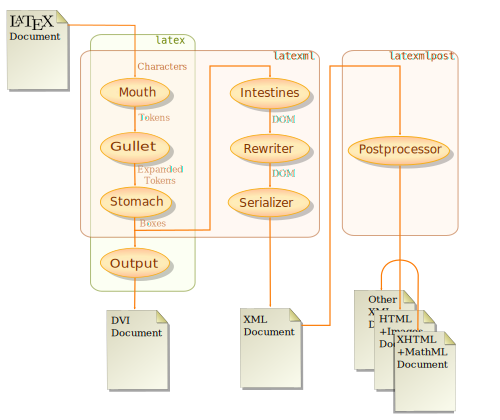
\includegraphics[width=\textwidth]{figures/digestion}
\end{center}
\caption{Flow of data through \LaTeXML's digestive tract.\label{architecture.dataflow}}
\end{figure}

The intention is that all semantics of the original document is
preserved by \ltxcmd{latexml}, or even inferred by parsing;
\ltxcmd{latexmlpost} is for formatting and conversion.
Depending on your needs, the \LaTeXML\ document resulting from \ltxcmd{latexml} may be
sufficient. Alternatively, you may want to enhance the document
by applying third party programs before postprocessing.

%%%----------------------------------------------------------------------
\section{latexml architecture}\label{architecture.latexml}
\index{LaTeXML!architecture}%
Like \TeX, \ltxcmd{latexml} is data-driven: the text and executable control
sequences (ie.~macros and primitives)
in the source file (and any packages loaded) direct the processing.
For \LaTeXML, the user exerts control over the conversion, and customizes it, by 
providing alternative bindings of the control sequences and packages,
by declaring properties of the desired document structure,
and by defining rewrite rules to be applied to the constructed document tree.

The top-level class, \pod{LaTeXML}, manages the processing, providing several methods
for converting a \TeX\ document or string into an \XML\ document, with varying degrees
of postprocessing and writing the document to file.
It binds a \ltxpod{Core::State} object (to \ltxcode|$STATE|)%$
to maintain the current state
of bindings for control sequence definitions and emulates \TeX's scoping rules.
The processing is broken into the following stages
\begin{description}
   \item[Digestion] the \TeX-like digestion phase which converts the input into boxes.
   \item[Construction] converts the resulting boxes into an \XML\ DOM.
   \item[Rewriting] applies rewrite rules to modify the DOM.
   \item[Math Parsing] parses the tokenized mathematics.
   \item[Serialization] converts the \XML\ DOM to a string, or writes to file.
\end{description}

%%%----------------------------------------------------------------------
\paragraph{Digestion}\label{architecture.latexml..digestion}
\index{Mouth(LaTeXML::)@{\ttfamily  Mouth(LaTeXML::)}!architecture}%
\index{Gullet(LaTeXML::)@{\ttfamily  Gullet(LaTeXML::)}!architecture}%
\index{Stomach(LaTeXML::)@{\ttfamily  Stomach(LaTeXML::)}!architecture}%
\index{Token(LaTeXML::)@{\ttfamily  Token(LaTeXML::)}!architecture}%
\index{Tokens(LaTeXML::)@{\ttfamily  Tokens(LaTeXML::)}!architecture}%
\index{Definition(LaTeXML::)@{\ttfamily  Definition(LaTeXML::)}!architecture}%
\index{Expandable(LaTeXML::)@{\ttfamily  Expandable(LaTeXML::)}!architecture}%
\index{Primitive(LaTeXML::)@{\ttfamily  Primitive(LaTeXML::)}!architecture}%
\index{Box(LaTeXML::)@{\ttfamily  Box(LaTeXML::)}!architecture}%
\index{List(LaTeXML::)@{\ttfamily  List(LaTeXML::)}!architecture}%
\index{Whatsit(LaTeXML::)@{\ttfamily  Whatsit(LaTeXML::)}!architecture}%

Digestion is carried out primarily in a \emph{pull} mode: The \ltxpod{Core::Stomach}
pulls expanded \ltxpod{Core::Token}s from the \ltxpod{Core::Gullet}, which itself pulls \ltxpod{Core::Token}s from 
the \ltxpod{Core::Mouth}.  The \ltxpod{Core::Mouth} converts characters from the plain text input
into \ltxpod{Core::Token}s according to the current \emph{catcodes} (category codes) assigned to
them (as bound in the \ltxpod{Core::State}).  
The \ltxpod{Core::Gullet} is responsible for expanding Macros,
that is, control sequences currently bound to \ltxpod{Core::Definition::Expandable}s
and for parsing sequences of tokens into common core datatypes
(\ltxpod{Common::Number}, \ltxpod{Common::Dimension}, etc.).
See \ref{customization.latexml.expansion} for how to define macros
and affect expansion.

The \ltxpod{Core::Stomach} then digests these tokens by executing \ltxpod{Core::Definition::Primitive} control 
sequences, usually for side effect, but often for converting material
into \ltxpod{Core::List}s of \ltxpod{Core::Box}es and \ltxpod{Core::Whatsit}s
(A Macro should never digest).
Normally, textual tokens are converted to \ltxpod{Core::Box}es in the current font.
The main (intentional) deviation of \LaTeXML's digestion from that of \TeX\ is
the introduction of a new type of definition, a \ltxpod{Core::Definition::Constructor},
responsible for constructing \XML\ fragments.
A control sequence bound to \ltxpod{Core::Definition::Constructor} is digested by
reading and processing its arguments and wrapping these up in a \ltxpod{Core::Whatsit}.
Before- and after-daemons, essentially anonymous primitives, associated with
the \ltxpod{Core::Definition::Constructor} are executed before and after digesting the \ltxpod{Core::Definition::Constructor}
arguments' markup, which can affect the context of that digestion, as well
as augmenting the \ltxpod{Core::Whatsit} with additional properties.
See \ref{customization.latexml.digestion} for how to define primitives
and affect digestion.


%%%----------------------------------------------------------------------
\paragraph{Construction}\label{architecture.latexml.construction}
\index{Constructor (LaTeXML::)!architecture}%
\index{Document (LaTeXML::)!architecture}%
\index{Model (LaTeXML::)!architecture}%
Given the \ltxpod{Core::List} of \ltxpod{Core::Box}es and \ltxpod{Core::Whatsit}s,
we proceed to constructing an \XML\ document.
This consists of creating an \ltxpod{Core::Document} object, containing
a libxml2 document, \pod{XML::LibXML::Document}, and having it absorb the digested
material. Absorbing a \ltxpod{Core::Box} converts it to text content, with provision
made to track and set the current font.
A \ltxpod{Core::Whatsit} is absorbed by invoking the associated \ltxpod{Core::Definition::Constructor}
to insert an appropriate \XML\ fragment, including elements and attributes,
and recursively processing their arguments as necessary
See \ref{customization.latexml.construction} for how to define
constructors.

A \ltxpod{Common::Model} is maintained througout the digestion phase which accumulates
any document model declarations, in particular the document type (RelaxNG is
preferred, but DTD is also supported).  As \LaTeX\ markup is more
like \SGML\ than \XML, additional declarations may be used (see \code{Tag} in \ltxpod{Package})
to indicate which elements may
be automatically opened or closed when needed to build a document tree that matches
the document type.  As an example, a \xmlcode{<subsection>} will automaticall be closed
when a \xmlcode{<section>} is begun.  Additionally, extra bits of code can
be executed whenever particularly elements are openned or closed (also
specified by \code{Tag}).
See \ref{customization.latexml.schema} for how to affect the schema.

%%%----------------------------------------------------------------------
\paragraph{Rewriting}\label{architecture.latexml.rewriting}
\index{Rewrite (LaTeXML::)!architecture}%
Once the basic document is constructed, \ltxpod{Core::Rewrite} rules are applied which can
perform various functions. Ligatures and combining mathematics digits and letters (in certain fonts)
into composite math tokens are handled this way.  Additionally, declarations
of the type or grammatical role of math tokens can be applied here
See \ref{customization.latexml.rewriting} for how to define rewrite rules.

%%%----------------------------------------------------------------------
\paragraph{MathParsing}\label{architecture.latexml.mathparsing}
\index{MathParser (LaTeXML::)!architecture}%
After rewriting, a grammar based parser is applied to the mathematical
nodes in order to infer, at least, the structure of the expressions,
if not the meaning.
Mathematics parsing, and how to control it, is covered in detail in Chapter \ref{math}.

%%%----------------------------------------------------------------------
\paragraph{Serialization}\label{architecture.latexml.serialization}
Here, we simple convert the DOM into string form, and output it.

%%%----------------------------------------------------------------------
\section{latexmlpost architecture}\label{architecture.latexmlpost}
\index{Post (LaTeXML::)!architecture}%
\LaTeXML's postprocessor is primarily for format conversion.
It operates by applying a sequence of filters responsible for
transforming or splitting documents, or their parts, from one format to another.

Exactly which postprocessing filter modules are applied depends
on the commandline options to \ltxcmd{latexmlpost}.
Postprocessing filter modules are generally applied in the following order:
\begin{description}
  \item[Split] splits the document into several `page' documents,
   according to \cmd{--split} or \cmd{--splitxpath} options.
  \item[Scan] scans the document for all ID's, labels and cross-references.
    This data may be stored in an external database,  depending on the \cmd{--db} option.
  \item[MakeIndex] fills in the \elementref{index} element (due to a \verb|\printindex|)
   with material generated by \verb|index|.
  \item[MakeBibliography] fills in the \elementref{bibliography} element
   (from \verb|\bibliography|) with material extracted from the
   file specified by the \cmd{--bibilography} option, for all \verb|\cite|'d items.
  \item[CrossRef] establishes all cross-references between documents and
   parts thereof, filling in the references with appropriate text for the hyperlink.
  \item[MathImages, MathML, OpenMath] performs various conversions of the
   internal Math representation.
  \item[PictureImages, Graphics, SVG] performs various graphics conversions.
  \item[XSLT] applies an XSLT transformation to each document.
  \item[Writer] writes the document to a file in the appropriate location.
\end{description}
See \ref{customization.latexmlpost} for how to customize the postprocessing.

%%%======================================================================
% \part{Intermediate}
%%%======================================================================
\chapter{Customization}\label{customization}
The processsing of the \LaTeX\ document, its  conversion into \XML\ and ultimately
to \XHTML\ or other formats can be customized in various ways, at
different stages of processing and in different levels of complexity.
Depending on what you are trying to achieve, some approaches may be easier
than others: Recall Larry Wall's adage ``There's more than one way to do it.''

By far, the easiest way to customize the style of the output is by modifying the CSS,
see \ref{customization.latexmlpost.css}, so that is the recommended way
when it applies.

The basic conversion from \TeX\ markup to \XML\ is done by
\ltxcmd{latexml}, and is obviously affected by the mapping between the \TeX\ markup
and the \XML\ markup.  This mapping is defined by macros, primitives and, of course,
constructors;  The mapping that is in force at any time is determined by the
\LaTeXML-specific implementations of the \TeX\ packages involved, what we call `bindings'.
Consequently, you can customize the conversion by modifying the
bindings used by \ltxcmd{latexml}.

Likewise, you extend \ltxcmd{latexml} by creating bindings for
\TeX\ styles that hadn't been covered.

Or by defining your own \TeX\ style file along with it's \LaTeXML\ binding.

In all these cases, you'll need the same skills: understanding and using
text, tokens, boxes and whatsits, as well as macros and macro expansion,
primitives and digestion, and finally whatsits and constructors.
Understanding \TeX\ helps; reading the \LaTeXML\ bindings in the distribution
will give an idea of how we use it.
%%%
%% Understand TeX;
%% to implement: Understand the style file!
%% Realize that people will misuse/abuse/stretch,
%% often getting below the level of the advertised interface.
%%%
To teach \LaTeXML\ about new macros, to implement bindings for a
package not yet covered, or to modify the way \TeX\ control sequences
are converted to \XML, you will want to look at \ref{customization.latexml}.
To modify the way that \XML\ is converted to other formats such as \HTML,
see \ref{customization.latexmlpost}.

A particularly powerful strategy when you have control over the
source documents is to develop a semantically oriented \LaTeX\ style file,
say \texttt{smacros.sty}, and then provide a \LaTeXML\ binding
as \texttt{smacros.sty.ltxml}. In the \LaTeX\ version, you may style
the terms as you like; in the \LaTeXML\ version, you could control
the conversion so as to preserve the semantics in the \XML.
If \LaTeXML's schema is insufficient, then you would need to extend it
with your own representation; although that is beyond the scope of
the current manual, see the discussion below in \ref{customization.latexml.schema}.
In such a case, you would also need to extend the \XSLT\ stylesheets,
as discussed in \ref{customization.latexmlpost.xslt}.

%%%----------------------------------------------------------------------
\section{LaTeXML Customization}\label{customization.latexml}
This layer of customization deals with modifying the way a \LaTeX\ document
is transformed into \LaTeXML's \XML, primarily through defining the way
that control sequences are handled.
In \ref{usage.conversion.loading} the loading of various bindings was
described.  The facilities described in the following subsections
apply in all such cases, whether used to customize the processing
of a particular document or to implement a new \LaTeX\ package.
We make no attempt to be comprehensive here; please consult
the documentation for \ltxpod{Global} and \ltxpod{Package},
as well as the binding files included with the system
for more guidance.

A \LaTeXML\ binding is actually a Perl module, and as such, 
a familiarity with Perl is helpful.
A binding file will look something like:
\begin{lstlisting}[style=latexml]
  use LaTeXML::Package;
  use strict;
  use warnings;
  # Your code here!

  1;
\end{lstlisting}
The final `1' is required; it tells Perl that the module has loaded successfully.
In between, comes any Perl code you wish, along with the definitions
and declarations as described here.

Actually, familiarity with Perl is more than merely helpful, as is familiarity
with \TeX\ and \XML! When writing a binding, you will be programming with all
three languages.  Of course, you need to know the \TeX\ corresponding to
the macros that you intend to implement, but sometimes it is most convenient
to implement them completely, or in part, in \TeX, itself (eg. using \ltxcode|DefMacro|),
rather then in Perl. At the other end, constructors (eg. using \ltxcode|DefConstructor|)
are usually defined by patterns of \XML.

\subsection[Expansion]{Expansion \& Macros}\label{customization.latexml.expansion}
%\paragraph{\texttt{DefMacro}}
\paragraph[DefMacro]{%
   \texttt{DefMacro(\textit{\$prototype},\textit{\$replacement},\textit{\%options})}}
Macros are defined using \texttt{DefMacro}, such as the pointless:
\begin{lstlisting}[style=latexml]
  DefMacro('\mybold{}','\textbf{#1}');
\end{lstlisting}
The two arguments to \texttt{DefMacro} we call
the \emph{prototype} and the \emph{replacement}.
In the prototype, the \verb|{}| specifies a single normal \TeX\ parameter.
The replacement is here a string which will
be tokenized and the \verb|#1| will be replaced by the
tokens of the argument. Presumably the entire result will
eventually be further expanded and or processed.

Whereas, \TeX\ normally uses \verb|#1|, and \LaTeX\ has developed
a complex scheme where it is often necessary to peek ahead token
by token to recognize optional arguments, we have attempted
to develop a suggestive, and easier to use, notation for parameters.
Thus a prototype \verb|\foo{}| specifies a single normal argument,
wheere \verb|\foo[]{}| would take an optional argument followed
by a required one.  More complex argument prototypes can be
found in \ltxpod{Package}.
As in \TeX, the macro's arguments are neither expanded
nor digested until the expansion itself is further
expanded or digested.

The macro's replacement can also be Perl code, typically an
anonymous \texttt{sub}, which gets the current \ltxpod{Core::Gullet}
followed by the macro's arguments as its arguments.  It must
return a list of \ltxpod{Core::Token}'s which will be used as the
expansion of the macro.  The following two examples show
alternative ways of writing the above macro:
\begin{lstlisting}[style=latexml]
  DefMacro('\mybold{}', sub {
    my($gullet,$arg)=@_;
    (T_CS('\textbf'),T_BEGIN,$arg,T_END); });
\end{lstlisting}
or alternatively
\begin{lstlisting}[style=latexml]
  DefMacro('\mybold{}', sub {
    Invocation(T_CS('\textbf'),$_[1]); });
\end{lstlisting}
Generally, the body of the macro should \emph{not} involve side-effects, assignments
or other changes to state other than reading \ltxpod{Core::Token}'s from the \ltxpod{Core::Gullet};
of course, the macro may expand into control sequences which do have side-effects.

\paragraph[Tokens, Catcodes,\ldots]{\texttt{Tokens}, Catcodes and friends}
Functions that are useful for dealing with \ltxpod{Core::Token}s and writing macros
include the following:
\begin{itemize}
\item Constants for the corresponding \TeX\ catcodes:
\begin{lstlisting}[style=latexml]
   CC_ESCAPE, CC_BEGIN,  CC_END,     CC_MATH,
   CC_ALIGN,  CC_EOL,    CC_PARAM,   CC_SUPER,
   CC_SUB,    CC_IGNORE, CC_SPACE,   CC_LETTER,
   CC_OTHER,  CC_ACTIVE, CC_COMMENT, CC_INVALID
\end{lstlisting}
%       \ltxcode|CC_CS|, \ltxcode|CC_NOTEXPANDED|
\item Constants for tokens with the appropriate content and catcode:
\begin{lstlisting}[style=latexml]
  T_BEGIN, T_END,   T_MATH,  T_ALIGN, T_PARAM,
  T_SUB,   T_SUPER, T_SPACE, T_CR
\end{lstlisting}
\item \ltxcode|T_LETTER($char)|, \ltxcode|T_OTHER($char)|, \ltxcode|T_ACTIVE($char)|,
  create tokens of the appropriate catcode with the given text content.
%     \ltxcode|T_COMMENT($string)|,
\item \ltxcode|T_CS($cs)| creates a control sequence token; 
  the string \ltxcode|$cs| should typically begin with the slash.
\item \ltxcode|Token($string,$catcode)| creates a token with the given content and catcode.
\item \ltxcode|Tokens($token,...)| creates a \ltxpod{Core::Tokens} object
   containing the list of \ltxpod{Core::Token}s.
\item \ltxcode|Tokenize($string)| converts the string to a \ltxpod{Core::Tokens},
   using \TeX's standard catcode assignments.
\item \ltxcode|TokenizeInternal($string)| like \texttt{Tokenize}, but
   treating \ltxcode|@| as a letter.
\item \ltxcode|Explode($string)| converts the string to a \ltxpod{Core::Tokens} where
   letter character are given catcode \ltxcode|CC_OTHER|.
\item \ltxcode|Expand($tokens| expands \ltxcode|$tokens| (a \ltxpod{Core::Tokens}), returning
  a \ltxpod{Core::Tokens}; there should be no expandable tokens in the result.
\item \ltxcode|Invocation($cstoken,$arg,...)| Returns a \ltxpod{Core::Tokens} representing
  the sequence needed to invoke \ltxcode|$cstoken| on the given arguments (each are %$
  \ltxpod{Core::Tokens}, or undef for an unsupplied optional argument).
\end{itemize}

% Are any of the keyword options worth bringing up?
% Probably I should at least mention that they are there...

\subsection[Digestion]{Digestion \& Primitives}\label{customization.latexml.digestion}
Primitives are processed during the digestion phase in the \ltxpod{Core::Stomach},
after macro expansion (in the \ltxpod{Core::Gullet}),
and before document construction (in the \ltxpod{Core::Document}).
Our primitives generalize \TeX's notion of primitive; they are used to implement
\TeX's primitives, invoke other side effects and to convert Tokens into Boxes,
in particular, Unicode strings in a particular font.

Here are a few primitives from \texttt{TeX.pool}:
\begin{lstlisting}[style=latexml]
  DefPrimitive('\begingroup',sub {
    $_[0]->begingroup; });
  DefPrimitive('\endgroup',  sub {
    $_[0]->endgroup; });
  DefPrimitiveI('\batchmode',     undef,undef);
  DefPrimitiveI('\OE', undef, "\x{0152}");
  DefPrimitiveI('\tiny',        undef, undef,
    font=>{size=>5});
\end{lstlisting}

Other than for implementing \TeX's own primitives,
\texttt{DefPrimitive} is needed less often than \texttt{DefMacro} or \texttt{DefConstructor}.
 The main thing to keep in mind
is that primitives are processed after macro expansion,
by the \ltxpod{Core::Stomach}.  They are most useful for
side-effects, changing the \ltxpod{Core::State}.

\paragraph[DefPrimitive]{%
  {\texttt{DefPrimitive(\textit{\$prototype},\textit{\$replacement},\texttt{\%options})}}}
The replacement is either a string which will be used to create
a Box in the current font, or can be code taking the \ltxpod{Core::Stomach}
and the control sequence arguments as argument; like macros, these arguments
are not expanded or digested by default, they must be explicitly digested if necessary.
The replacement code must either return nothing (eg. ending with \ltxcode|return;|) or
should return a list (ie. a Perl list \ltxcode|(...)|)
of digested \ltxpod{Core::Box}es or \ltxpod{Core::Whatsit}s.

Options to DefPrimitive are:
\begin{itemize}
\item \ltxcode.mode=>('math'|'text'). switches to math or text mode, if needed;
\item \ltxcode|requireMath=>1|, \ltxcode|forbidMath=>1| requires, or forbids,
  this primitive to appear in math mode;
\item \ltxcode|bounded=>1| specifies that all digestion (of arguments and daemons)
  will take place within an implicit \TeX\ group, so that any side-effects
  are localized, rather than affecting the global state;
\item \ltxcode|font=>{%hash}|
  switches the font used for any created text;
  recognized font keys are \texttt{family}, \texttt{series}, \texttt{shape}, \texttt{size}, \texttt{color};
  
  Note that if the font change should only affect the material digested within this
  command itself, then \ltxcode|bounded=>1| should be used; otherwise, the font
  change will remain in effect after the command is processed.
\item \ltxcode|beforeDigest=>CODE($stomach)|,\\
      \ltxcode|afterDigest=>CODE($stomach)|
  provides code to be digested before and after processing
  the main part of the primitive.
\end{itemize}

% DefRegister ?
\paragraph[DefRegister]{%
    \textit{DefRegister(\ldots)}}
Needs descrition!

\paragraph[Other]{Other Utilities for Digestion}

Other functions useful for dealing with digestion and state are important for
writing before \& after daemons in constructors, as well as in Primitives;
we give an overview here:
\begin{itemize}
\item \ltxcode|Digest($tokens)|
digests \ltxcode|$tokens| (a \ltxpod{Core::Tokens}), returning a list of \ltxpod{Core::Box}es and \ltxpod{Core::Whatsit}s.
\item \ltxcode|Let($token1,$token2)| gives \ltxcode|$token1| the same meaning as \ltxcode|$token2|,
 like \verb|\let|.
\end{itemize}

\paragraph{Bindings} The following functions are useful for accessing and storing
information in the current \ltxpod{Core::State}. It maintains a stack-like structure
that mimics \TeX's approach to binding; braces \verb|{| and \verb|}| open
and close stack frames.  (The \ltxpod{Core::Stomach} methods \texttt{bgroup} and \texttt{egroup}
can be used when explicitly needed.)
\begin{itemize}
\item \ltxcode|LookupValue($symbol)|, \ltxcode|AssignValue($string,$value,$scope)|
 maintain arbitrary values in the current \ltxpod{Core::State}, looking up or assigning
 the current value  bound to \ltxcode|$symbol| (a string).
 For assignments,  the \ltxcode|$scope| can be \texttt{'local'}
  (the default, if \ltxcode|$scope| is omitted),
  which changes the binding in the current stack frame.
  If \ltxcode|$scope| is \texttt{'global'}, it assigns the value globally
  by undoing all bindings.
  The \ltxcode|$scope| can also be another string, which indicates a named scope
   --- but that is a more advanced topic.
\item \ltxcode|PushValue($symbol,$value,...)|, \ltxcode|PopValue($symbol)|,\hfil\\
      \ltxcode|UnshiftValue($symbol,$value,...)|, \ltxcode|ShiftValue($symbol)|
  These maintain the value of \ltxcode|$symbol| as a list, with the operatations
  having the same sense as in Perl; modifications are always global.
\item \ltxcode|LookupCatcode($char)|, \ltxcode|AssignCatcode($char,$catcode,$scope)|
  maintain the catcodes associated with characters.
\item \ltxcode|LookupMeaning($token)|, \ltxcode|LookupDefinition($token)|
 looks up the current meaning of the token,  being any executable definition bound for it.
 If there is no such defniition \texttt{LookupMeaning} returns the token itself, 
 \texttt{LookupDefinition} returns \texttt{undef}.
%  \ltxcode|InstallDefinition()|
\end{itemize}

\paragraph{Counters}
% Should this go under Constructors?
The following functions maintain \LaTeX-like counters, and generally
also associate an \texttt{ID} with them.  A counter's print form
(ie. \verb|\theequation| for equations) often ends up on the \attr{refnum} attribute
of elements; the associated \texttt{ID} is used for the \attr{xml:id} attribute.
\begin{itemize}
\item \ltxcode|NewCounter($name,$within,%options)|,
  creates a \LaTeX-style counters.  When \ltxcode|$within| is used, 
  the given counter will be reset whenever the counter \ltxcode|$within| is incremented.
  This also causes the associated \texttt{ID} to be prefixed with \ltxcode|$within|'s \texttt{ID}.
  The option \ltxcode|idprefix=>$string| causes the \texttt{ID} to be prefixed with that string.
  For example,
\begin{lstlisting}[style=latexml]
  NewCounter('section', 'document', idprefix=>'S');
  NewCounter('equation','document', idprefix=>'E',
    idwithin=>'section');
\end{lstlisting}
would cause the third equation in the second section to have \xmlcode{ID='S2.E3'}.
\item  \ltxcode|CounterValue($name)| returns the \ltxpod{Common::Number} representing the current value.
\item  \ltxcode|ResetCounter($name)| resets the counter to 0.
\item \ltxcode|StepCounter($name)| steps the counter (and resets any others `within' it),
  and returns the expansion of \verb|\the$name|.
\item \ltxcode|RefStepCounter($name)| steps the counter and any ID's associated with it.
  It returns a hash containing \texttt{refnum} (expansion of \verb|\the$name|)
  and \texttt{id} (expansion of \verb|\the$name@ID|)
\item \ltxcode|RefStepID($name)| steps the ID associated with the counter, without
  actually stepping the counter; this is useful for unnumbered units that normally
  would have both a refnum and ID.
%\ltxcode|GenerateID()|
\end{itemize}

\subsection[Construction]{Construction \& Constructors}\label{customization.latexml.construction}
Constructors are where things get interesting, but also complex; they are
responsible for defining how the \XML\ is built.  There are basic
constructors corresponding to normal control sequences, as well as
environments. Mathematics generally comes down to constructors, as well,
but is covered in Chapter \ref{math}.

Here are a couple of trivial examples of constructors:
\begin{lstlisting}[style=latexml]
  DefConstructor('\emph{}',
   "<ltx:emph>#1</ltx:emph>", mode=>'text');
  DefConstructor('\item[]',
    "<ltx:item>?#1(<ltx:tag>#1</ltx:tag>)");
  DefEnvironment('{quote}',   
    '<ltx:quote>#body</ltx:quote>',
    beforeDigest=>sub{ Let('\\\\','\@block@cr');});
  DefConstructor('\footnote[]{}',
    "<ltx:note class='footnote' mark='#refnum'>#2</ltx:note>",
    mode=>'text',
    properties=> sub { 
      ($_[1] ? (refnum=>$_[1]) : RefStepCounter('footnote')) });
\end{lstlisting}

\paragraph[DefConstructor]{%
   \texttt{DefConstructor(\textit{\$prototype},\textit{\$replacement},\textit{\%options})}}
The \ltxcode|$replacement| for a constructor describes the \XML\ to %$
be generated during the construction phase. It can either be a string
representing the \emph{XML pattern} (described below), or a
subroutine \ltxcode|CODE($document,$arg1,...%props)|
receiving the arguments and properties from the \ltxpod{Core::Whatsit};
it would invoke the methods of \ltxpod{Core::Document} to construct the desired \XML.

At its simplest, the XML pattern is a just serialization of the desired \XML.
For more expressivity, \XML\ trees, text content, attributes and attribute values can
be effectively `interpolated' into the \XML\ being constructed by use of the following expressions:
\begin{itemize}
\item \ltxcode|#1|,\ltxcode|#2|,\ldots \ltxcode|#%name%|
   returns the construction of the numbered argument
   or named property of the Whatsit;
\item \ltxcode|&%function%(%arg1%,%arg2%,...)|
   invokes the Perl \codevar{function} on the given arguments,
   \codevar{arg1},\ldots, returning the result.
   The arguments should be expressions for values, rather than \XML\ subtrees.
\item \ltxcode|?%test%(%if pattern%)| 
   or \ltxcode|?%test%(%if pattern%)(%else pattern%)|
   returns the result of either the \codevar{if} or \codevar{else} pattern
   depending on whether the result of \codevar{test} (typically also an expression) is non-empty;
\item \verb|%|\ltxcode
   returns a hash (or rather assumes the result is a hash or KeyVals object);
   this is only allowed within an opening \XML\ tag, where all the key-value pairs are
   inserted as attributes;
\item \ltxcode|^|
   if this appears at the beginning of the pattern,
   the replacement is allowed to \emph{float} up the current tree to whereever it might be allowed;
\end{itemize}
In each case, the result of an expression is expected to be either an \XML\ tree,
a string or a hash, depending on the context it was used in.  In particular,
values of attributes are typically given by quoted strings, but expressions within those
strings are interpolated into the computed attribute value.
The special characters \verb|@ # ? %| which introduce these expressions can
be escaped by preceding with a backslash, when the literal character is desired.

A subroutine used as the \ltxcode|$replacement|, %$
allows programmatic insertion of \XML\ into, or modification of, the document being constructed.
Although one could use LibXML's DOM API to manipulate the document tree,
it is \emph{strongly} recommended to use \ltxpod{Core::Document}'s API whereever possible
as it maintains consistency and manages namespace prefixes.
This is particularly true for insertion of new content, setting attributes and
finding existing nodes in the tree using XPath. 

Options:
\begin{itemize}
\item \ltxcode.mode=>('math'|'text'). switches to math or text mode, if needed;
\item \ltxcode|requireMath=>1|, \ltxcode|forbidMath=>1| requires, or forbids,
  this constructor to appear in math mode;
\item \ltxcode|bounded=>1| specifies that all digestion (of arguments and daemons)
  will take place within an implicit \TeX\ group, so that any side-effects
  are localized, rather than affecting the global state;
\item \ltxcode|font=>{%hash}|
  switches the font used for any created text;
  recognized font keys are \texttt{family}, \texttt{series}, \texttt{shape}, \texttt{size},
  \texttt{color};
\item \ltxcode.properties=> {%hash} | CODE($stomach,$arg1,...).
  provides a set of properties to store in the \ltxpod{Core::Whatsit} for eventual use
  in the constructor \ltxcode|$replacement|.  If a subroutine is used,
  it also should return a hash of properties;
\item \ltxcode|beforeDigest=>CODE($stomach)|,\\
      \ltxcode|afterDigest=>CODE($stomach,$whatsit)|
  provides code to be digested before and after digesting the arguments of
  the constructor, typically to alter the context of the digestion (before),
  or to augment the properties of the \ltxpod{Core::Whatsit} (after);
\item  \ltxcode|beforeConstruct=>CODE($document,$whatsit)|,\\
      \ltxcode|afterConstruct=>CODE($document,$whatit)|
  provides code to be run before and after the main \ltxcode|$replacement|
  is effected; occassionaly it is convenient to use the pattern
  form for the main \ltxcode|$replacement|, but one still wants to execute
  a bit of Perl code, as well;
%\item \ltxcode|nargs|  HUH?
\item \ltxcode.captureBody=>(1 | $token).
  specifies that an additional argument (like an environment body) wiil
  be read until the current \TeX\ grouping ends, or until the specified \ltxcode|$token|
  is encountered. This argument is available to \ltxcode|$replacement| as \ltxcode|$body|;
\item \ltxcode.scope=>('global'|'local'|$name). specifies whether this
  definition is made globally, or in the current stack frame (default),
  (or in a named scope);
\item \ltxcode&reversion=>$string|CODE(...)&,
   \ltxcode|alias=>$cs|
  can be used when the \ltxpod{Core::Whatsit} needs to be reverted into \TeX\ code,
  and the default of simply reassembling based on the prototype is not desired.
  See the code for examples.
\end{itemize}

Some additional functions useful when writing constructors:
\begin{itemize}
\item \ltxcode|ToString($stuff)| converts \ltxcode|$stuff| to a string,
  hopefully without \TeX\ markup, suitable for use as document content
  and attribute values.  Note that if \ltxcode|$stuff| contains Whatsits
  generated by Constructors, it may not be possible to avoid \TeX\ code.
  Constrast \ltxcode|ToString| to the following two functions.
\item \ltxcode|UnTeX($stuff)| returns a string containing the \TeX\ code
  that would generate \ltxcode|$stuff| (this might not be the original \TeX).
  The function \ltxcode|Revert($stuff)| returns the same information as a Tokens list.
\item \ltxcode|Stringify($stuff)| returns a string more intended
  for debugging purposes; it reveals more of the structure and type information
  of the object and its parts.
\item \ltxcode|CleanLabel($arg)|,
   \ltxcode|CleanIndexKey($arg)|,
   \ltxcode|CleanBibKey($arg)|,\hfil\\
   \ltxcode|CleanURL($arg)|
  cleans up arguments (converting to string, handling invalid characters, etc)
  to make the argument appropriate for use as an attribute representing
  a label, index ID, etc.
\item \ltxcode|UTF($hex)| returns the Unicode character for the given
codepoint; this is useful for characters below \texttt{0x100} where
Perl becomes confused about the encoding.
\end{itemize}

\paragraph[DefEnvironment]{%
  \textit{DefEnvironment(\textit{\$prototype},\textit{\$replacement},\textit{\%options})}}
Environments are largely a special case of constructors,
but the prototype starts with \verb|{envname}|, rather than \verb|\cmd|,
the replacement will also typically involve \verb|#body| representing
the contents of the environment.

\texttt{DefEnvironment} takes the same options as  \texttt{DefConstructor},
with the addition of
\begin{itemize}
\item \ltxcode|afterDigestBegin=>CODE($stomach,$whatsit)|
provides code to digest after the \verb|\begin{env}| is digested;
\item \ltxcode|beforeDigestEnd=>CODE($stomach)|
provides code to digest before the \verb|\end{env}| is digested.
\end{itemize}

For those cases where you do not want an environment to correspond
to a constructor, you may still (as in \LaTeX), define the
two control sequences \verb|\envname| and \verb|\endenvname|
as you like.

\subsection{Document Model}\label{customization.latexml.schema}
The following declarations are typically only needed when customizing
the schema used by \LaTeXML.
\begin{itemize}
\item \ltxcode|RelaxNGSchema($schema,%namespaces)| declares the created
 \XML\ document should be fit to the RelaxNG schema in \ltxcode|$schema|;
 A file \ltxcode|$schema.rng| should be findable in the current search paths.
(Note that currently, \LaTeXML\ is unable to directly parse compact notation).
\item \ltxcode|RegisterNamespace($prefix,$url)| associates the
 prefix with the given namespace url.  This allows you to use \ltxcode|$prefix|
 as a namespace prefix when writing \ltxpod{Core::Definition::Constructor} patterns or XPath expressions.
\item \ltxcode|Tag($tag,%properties)| specifies properties for the given \XML\ \ltxcode|$tag|.
Recognized properties include:
\ltxcode|autoOpen=>1| indicates that the tag
can automatically be opened if needed to create a valid document;
\ltxcode|autoClose=>1| indicates that the tag can automatically be closed if needed to create
a valid document;
\ltxcode|afterOpen=>$code| specifies code to be executed before opening the tag;
the code is passed the \ltxpod{Core::Document} being constructed as well as the
\ltxpod{Core::Box} (or \ltxpod{Core::Whatsit}) responsible for its creation;
\ltxcode|afterClose=>code| similar to \texttt{afterOpen}, but executed after closing
the element.
% DocType
\end{itemize}

\subsection{Rewriting}\label{customization.latexml.rewriting}
The following functions are a bit tricky to use (and describe),
but can be quite useful in some circumstances.

\paragraph[DefLigature]{%
    \texttt{DefLigature(\textit{\$regexp},\textit{\%options})}}
applies a regular expression
to substitute textnodes after they are closed; the only option is \ltxcode|fontTest=>$code|
which restricts the ligature to text nodes where the current font passes \ltxcode|&$code($font)|.

\paragraph[DefMathLigature]{%
    \texttt{DefMathLigature(\textit{\$code},\textit{\%options})}}
allows replacement of sequences of math nodes.
It applies \ltxcode|$code| to the current \ltxpod{Core::Document}
and each sequence of math nodes encountered in the document; if a replacement should
occur, \ltxcode|$code| should return a list of the form \ltxcode|($n,$string,%attributes)|
in which case, the text content of the first node is replaced by \ltxcode|$string|,
the given attributes are added, and the following \ltxcode|$n-1| nodes are removed.

\paragraph[DefRewrite]{%
  \textit{DefRewrite(\textit{\%spec})}}
defines document rewrite rules. These specifications describe what document nodes match:
\begin{itemize}
\item \ltxcode|label=>$label| restricts to nodes contained within an element whose
  \attr{labels} includes \ltxcode|$label|;
\item \ltxcode|scope=>$scope| generalizes \texttt{label}; the most useful form
 a string like \texttt{'section:1.3.2'} where it matches the \elementref{section}
  element whose \attr{refnum} is \texttt{1.3.2};
\item \ltxcode|xpath=>$xpath| selects nodes matching the given XPath;
\item \ltxcode|match=>$tex| selects nodes that look like what processing
 the \TeX\ string \ltxcode|$tex| would produce;
\item \ltxcode|regexp=>$regexp| selects text nodes that match the given regular expression.
\end{itemize}
The following specifications describe what to do with the matched nodes:
\begin{itemize}
\item \ltxcode|attributes=>{%attr}| adds the given attributes to the matching nodes;
\item \ltxcode|replace=>$tex| replaces the matching nodes with the result
of processing the \TeX\ string \ltxcode|$tex|.
\end{itemize}

\subsection{Packages and Options}\label{customization.latexml.packages}
The following declarations are useful for defining \LaTeXML\ bindings,
including option handling.
As when defining \LaTeX\ packages, the following, if needed at all,
need to appear in the order shown.
\begin{itemize}
%===== Declarations of options
\item \ltxcode|DeclareOption($option,$handler)| specifies the handler
for \ltxcode|$option| when it is passed to the current package or class.
If \ltxcode|$option| is \texttt{undef}, it defines the default handler,
for options that are otherwise unrecognized.
\ltxcode|$handler| can be either a string to be expanded, or a sub which
is executed like a primitive.
\item \ltxcode|PassOptions($name,$type,@options)|  specifies that the
given options should be passed to the package (if \ltxcode|$type| is \texttt{sty})
or class (if \ltxcode|$type| is \texttt{cls}) \ltxcode|$name|, if it is ever loaded.
%===== Execution of options
\item \ltxcode|ProcessOptions(%keys)| processes any options that have
been passed to the current package or class.  If \ltxcode|inorder=>1| is
specified, the options will be processed in the order passed to the
package (\verb|\ProcessOptions*|); otherwise they will be processed
in the declared order (\verb|\ProcessOptions|).
\item \ltxcode|ExecuteOptions(@options)|
executes the handlers for the specific set of options \ltxcode|@options|.
%===== Package loading
\item \ltxcode|RequirePackage($pkgname,%keys)| loads the specified package.
The keyword options have the following effect: \ltxcode|options=>$options|
can provide an explicit array of string specifying the options to pass to the package;
\ltxcode|withoptions=>1| means that the options passed to the currently loading
class or package should be passed to the requested package;
\ltxcode|type=>$ext| specifies the type of the package file (default is \texttt{sty});
\ltxcode|raw=>1| specifies that reading the raw style file (eg. \texttt{pkg.sty})
is permissible if there is no specific \LaTeXML\ binding (eg. \texttt{pkg.sty.ltxml})
\ltxcode|after=>$after| specifies a string or \ltxpod{Core::Tokens} to be expanded
after the package has finished loading.
\item \ltxcode|LoadClass($classname,%keys)|
Similar to \texttt{RequirePackage}, but loads a class file (\ltxcode|type=>'cls'|).
%==== Special commands
\item \ltxcode|AddToMacro($cstoken,$tokens)| a little used utilty to add
material to the expansion of \ltxcode|$cstoken|, like an \verb|\edef|;
typically used to add code to a class or package hook.
\end{itemize}

\subsection{Miscellaneous}\label{customization.latexml.misc}
Other useful stuff:
\begin{itemize}
\item \ltxcode|RawTeX($texstring)| expands and processes the \ltxcode|$texstring|;
This is typically useful to include definitions copied from a \TeX\ stylefile,
when they are approriate for \LaTeXML, as is.
Single-quoting the \ltxcode|$texstring| is useful, since it isn't interpolated
by Perl, and avoids having to double all the slashes!
\end{itemize}

%\ltxcode|MergeFont()|

%%%----------------------------------------------------------------------
\section{latexmlpost Customization}\label{customization.latexmlpost}
The current postprocessing framework works by passing the document through
a sequence of postprocessing filter modules. Each module is responsible
for carrying out a specific transformation, augmentation or conversion
on the document.   In principle, this architecture has the flexibility to
employ new filters to perform new or customized conversions.
However, the driver, \ltxcmd{latexmlpost}, currently provides no
convenient means to instanciate and incorporate outside filters, short
of developing your own specialized version.

Consequently, we will consider custom postprocessing filters outside
the scope of this manual (but of course, you are welcome to explore
the code, or contact us with suggestions).

The two areas where customization is most practical is in altering
the XSLT transforms used and extending the \CSS\ stylesheets.

\subsection{XSLT}\label{customization.latexmlpost.xslt}
\LaTeXML\ provides stylesheets for transforming its \XML\ format
to \XHTML\ and \HTML. These stylesheets are modular with components
corresponding to the schema modules.  Probably the best strategy
for customizing the transform involves making a copy of the standard
base stylesheets, \texttt{LaTeXML-xhtml.xsl},
\texttt{LaTeXML-html.xsl} and
\texttt{LaTeXML-html5.xsl},  found at
\textit{installationdir}\texttt{/LaTeXML/style/}
--- they're short, consisting mainly of an \texttt{xsl:include}
and setting appropriate parameters and output method;
thus modifying the parameters and and adding your own rules,
or including your own modules should be relatively easy.

Naturally, this requires a familiarity with \LaTeXML's schema (see \ref{schema}),
as well as \XSLT\ and \XHTML.  See the other stylesheet modules in the same directory
as the base stylesheet for guidance.
Generally the strategy is to use various parameters to switch
between common behaviors and to use templates with \texttt{mode}s
that can be overridden in the less common cases.

Conversion to formats other than \XHTML\ are, of course, possible, as well,
but are neither supplied nor covered here.
How complex the transformation will be depends on the extent
that the \LaTeXML\ schema can be mapped to the desired one,
and to what extent \LaTeXML\ has lost or hidden information
represented in the original document.  Again, familiarity with the schema is needed,
and the provided \XHTML\ stylesheets may suggest an approach.

NOTE: I'm trying to make stylesheets \emph{easily} customizable.
However, this is getting tricky.
\begin{itemize}
\item You can import stylesheets which allows the templates to be overridden.
\item You can call the overridden stylesheet using \texttt{apply-imports}
\item You can \emph{not} call \texttt{apply-imports} to call an overridden
\emph{named} template! (although you seemingly can override them?)
\item You can refer to xslt modules using URN's, provided you have loaded
the \texttt{LaTeXML.catalog}:
{\small
\begin{lstlisting}[style=xml]
<xsl:import href="urn:x-LaTeXML:XSLT:LaTeXML-all-xhtml.xsl"/>
\end{lstlisting}
}
\end{itemize}

\subsection{CSS}\label{customization.latexmlpost.css}
\CSS\ stylesheets can be supplied to \ltxcmd{latexmlpost} to
be included in the generated documents in addition to, or as a
replacement for, the standard stylesheet \texttt{LaTeXML.css}.
See the directory
\textit{installationdir}\texttt{/LaTeXML/style/}
for samples.

To best take advantage of this capability so as to design
\CSS\ rules with the correct specificity, the following points are helpful:
\begin{itemize}
\item \LaTeXML\ converts the \TeX\ to its own schema,
  with structural elements (like \elementref{equation}) getting their own tag;
  others are transformed to something more generic, such as \elementref{note}.
  In the latter case, a class attribute is often used to distinguish.
  For example, a \verb|\footnote| generates
\begin{lstlisting}[style=xml]
  <note class='footnote'>...
\end{lstlisting}
  whereas an \verb|\endnote| generates
\begin{lstlisting}[style=xml]
  <note class='endnote'>...
\end{lstlisting}
\item The provided \XSLT\ stylesheets transform \LaTeXML's schema to \XHTML,
  generating a combined class attribute consisting of any class attributes
  already present as well as the \LaTeXML\ tag name.
  However, there are some variations on the theme.
  For example, \LaTeX's \verb|\section| yeilds a \LaTeXML\ element \elementref{section},
  with a \elementref{title} element underneath.  When transformed to
  \XHTML, the former becomes a \xmlcode{<div class='section'>},
  while the latter becomes \xmlcode{<h2 class='section-title'>}
 (for example, the h-level may vary with the document structure),
\end{itemize}

\paragraph{Mode \texttt{begin} and \texttt{end}}
For most elements, once the main html element has been opened and the
primary attributes have been added but before any content has been added,
a template with mode \texttt{begin} is called;
thus it can add either attributes or content.  Just before closing the main
html element, a template with mode \texttt{end} is called.

\paragraph{Computing class and style}
Templates with mode \texttt{classes} and \texttt{styling}.

%%%======================================================================
\chapter{Mathematics}\label{math}

%\ltxcode|DefMath($prototype,$replacement,%options)|

There are several issues that have to be dealt with in treating the mathematics.
On the one hand, the \TeX\ markup gives a pretty good indication of what the
author wants the math to look like, and so we would seem to have a good handle
on the conversion to presentation forms.  On the other hand, content formats
are desirable as well; there are a few, but too few, clues about what the
intent of the mathematics is.  And in fact, the generation of even Presentation
MathML of high quality requires recognizing the mathematical structure, if not
the actual semantics. The mathematics processing must therefore preserve the
presentational information provided by the author, while inferring, likely
with some help, the mathematical content.

From a parsing point of view, the \TeX-like processing serves as the lexer,
tokenizing the input which \LaTeXML\ will then parse
[perhaps eventually a type-analysis phase will be added].
Of course, there are a few twists.
For one, the tokens, represented by \elementref{XMTok}, can carry extra attributes
such as font and style, but also the name, meaning and grammatical role,
with defaults that can be overridden by the author --- more on those, in a moment.
Another twist is that, although \LaTeX's math markup is not nearly
as semantic as we might like, there is considerable semantics and structure in the 
markup that we can exploit. For example, given a \verb|\frac|, we've already
established the numerator and denominator which can be parsed individually,
but the fraction as a whole can be directly represented as an application,
using \elementref{XMApp}, of a fraction operator; the resulting structure can be treated
as atomic within its containing expression.This \emph{structure preserving} character
greatly simplifies the parsing task and helps reduce misinterpretation.

The parser, invoked by the postprocessor, works only with the top-level lists of lexical tokens,
or with those sublists contained in an \elementref{XMArg}.  The grammar works primarily through
the name and grammatical role.  The name is given by an attribute, or the content if it is
the same.  The role (things like ID, FUNCTION, OPERATOR, OPEN, \ldots) is also given
by an attribute, or, if not present, the name is looked up in a document-specific
dictionary (\varfile[dict]{jobname}), or in a default dictionary.

Additional exceptions that need fuller explanation are: 
\begin{itemize}
 \item \ltxpod{Core::Definition::Constructor}s may wish to create a dual object (\elementref{XMDual}) whose children are 
the semantic and presentational forms.
 \item Spacing and similar markup generates \elementref{XMHint} elements, which are currently ignored
during parsing, but probably shouldn't.
\end{itemize}

%%%----------------------------------------------------------------------
\section{Math Details}\label{math.details}
\LaTeXML\ processes mathematical material by proceeding through several stages:
\begin{itemize}
\item Basic processing of macros, primitives and constructors resulting in
   an XML document; the math is primarily represented by a sequence of
   tokens (\elementref{XMTok}) or structured items (\elementref{XMApp}, \elementref{XMDual}) and
   hints (\elementref{XMHint}, which are ignored).
\item Document tree rewriting, where rules are applied to modify the document tree.
   User supplied rules can be used here to clarify the intent of markup used in the document.
\item Math Parsing; a grammar based parser is applied, depth first, to each level of the math.
   In particular, at the top level of each math expression, as well as each
   subexpression within structured items (these will have been contained in
   an \elementref{XMArg} or \elementref{XMWrap} element).  This results in an expression tree
   that will hopefully be an accurate representation of the expression's structure,
   but may be ambigous in specifics (eg. what the meaning of a superscript is).
   The parsing is driven almost entirely by the grammatical \attr{role} assigned
   to each item.
\item \emph{Not yet implemented} a following stage must be developed to resolve
   the semantic ambiguities by analyzing and augmenting the expression tree.
\item Target conversion: from the internal \texttt{XM*} representation to
   \MathML\ or \OpenMath.
\end{itemize}

The \elementref{Math} element is a top-level container for any math mode material,
serving as the container for various representations of the math including
images (through attributes \attr{mathimage}, \attr{width} and \attr{height}), 
textual (through attributes \attr{tex}, \attr{content-tex} and \attr{text}),
\MathML\ and the internal representation itself.  
The \attr{mode} attribute specifies whether the math should be in display or inline mode.

\subsection{Internal Math Representation}\label{math.details.representation}
The \elementref{XMath} element is the container for the internal representation

The following attributes can appear on all \texttt{XM*} elements:
\begin{description}
\item[\attr{role}] the grammatical role that this element plays 
\item[\attr{open}, \attr{close}] parenthese or delimiters that were used to wrap the
   expression represented by this element.
\item[\attr{argopen}, \attr{argclose}, \attr{separators}] delimiters on an function or operator
   (the first element of an \elementref{XMApp})  that were used to delimit the arguments of the function.
    The separators is a string of the punctuation characters used to separate arguments.
\item[\attr{xml:id}] a unique identifier to allow reference (\elementref{XMRef}) to this element.
\end{description}

\paragraph{Math Tags} The following tags are used for the intermediate math representation:
\begin{description}
\item[\elementref{XMTok}] represents a math token. It may contain text for presentation.
   Additional attributes are:
  \begin{description}
   \item[\attr{name}] the name that represents the \emph{meaning} of the token; this overrides
      the content for identifying the token.
   \item[\attr{omcd}] the \OpenMath\ content dictionary that the name belongs to.
   \item[\attr{font}] the font to be used for presenting the content.
   \item[\attr{style}] ?
   \item[\attr{size}] ?
   \item[\attr{stackscripts}] whether scripts should be stacked above/below the item, instead
     of the usual script position.
  \end{description}
\item[\elementref{XMApp}] represents the generalized application of some function or operator to arguments.
   The first child element is the operator, the remainig elements are the arguments.
   Additional attributes:
  \begin{description}
    \item[\attr{name}] the name that represents the meaning of the construct as a whole.
    \item[\attr{stackscripts}] ?
  \end{description}
\item[\elementref{XMDual}] combines representations of the content (the first child) and presentation
   (the second child), useful when the two structures are not easily related.
\item[\elementref{XMHint}] represents spacing or other apparent purely presentation material.
  \begin{description}
    \item[\attr{name}] names the effect that the hint was intended to achieve.
    \item[\attr{style}] ?
  \end{description}
\item[\elementref{XMWrap}] serves to assert the expected type or role of a subexpression that
  may otherwise be difficult to interpret --- the parser is more forgiving about these.
  \begin{description}
    \item[\attr{name}] ?
    \item[\attr{style}] ?
  \end{description}
\item[\elementref{XMArg}] serves to wrap individual arguments or subexpressions, created by
  structured markup, such as \verb|\frac|.  These subexpressions can be parsed individually.
  \begin{description}
    \item[\attr{rule}] the grammar rule that this subexpression should match.
  \end{description}
\item[\elementref{XMRef}] refers to another subexpression,.  This is used to avoid duplicating
  arguments when constructing an \elementref{XMDual} to represent a function application, for example.  
  The arguments will be placed in the content branch (wrapped in an \elementref{XMArg}) while
  \elementref{XMRef}'s will be placed in the presentation branch.
  \begin{description}
    \item[\attr{idref}] the identifier of the referenced math subexpression.
  \end{description}
\end{description}

\subsection{Grammatical Roles}\label{math.details.roles}
As mentioned above, the grammar take advantage of the structure (however minimal) of the markup.
Thus, the grammer is applied in layers, to sequences of tokens or \emph{atomic} 
subexpressions (like a fractions or arrays). It is the \attr{role} attribute
that indicates the syntactic and/or presentational nature of each item.
On the one hand, this drives the parsing: the grammar rules are keyed
on the \attr{role} (say, \code{ADDOP}), rather than content (say + or -), of the nodes
[In some cases, the content is used to distinguish special synthesized roles].
The \attr{role} is also used to drive the conversion to presentation markup, 
(say, as an infix operator), especially Presentation \MathML.
Some values of \attr{role} are used only in the grammar,
some are only used in presentation; most are used both ways.

The following grammatical roles are recognized by the math parser.
These values can be specified in the \attr{role} attribute during the initial 
document construction or by rewrite rules.  Although the precedence of operators
is loosely described in the following, since the grammar contains various special
case productions, no rigidly ordered precedence is given.
Also note that in the current design, an expresssion has only a single role,
although that role may be involved in grammatical rules with distinct syntax and semantics
(some roles directly reflect this ambiguity).
\begin{description}
\item[\code{ATOM}] a general atomic subexpression
  (atomic at the level of the expression; it may have internal structure);
\item[\code{ID}] a variable-like token, whether scalar or otherwise,
  but not a function;
\item[\code{NUMBER}] a number;
\item[\code{ARRAY}] a structure with internal components and alignments;
  typically has a particular syntactic relationship to \code{OPEN} and \code{CLOSE} tokens.
\item[\code{UNKNOWN}] an unknown expression. This is the default for token elements.
  Such tokens are treated essential as \code{ID}, but generate a warning if it
  seems to be used as a function.

\item[\code{OPEN},\code{CLOSE}] opening and closing delimiters, group expressions
  or enclose arguments among other structures;
\item[\code{MIDDLE}] a middle operator used to group items between an \code{OPEN},
  \code{CLOSE} pair;
\item[\code{PUNCT},\code{PERIOD}] punctuation; a period `ends' formula
  (note that numbers, including floating point, are recognized earlier in processing);
\item[\code{VERTBAR}] a vertical bar (single or doubled) which serves a confusing variety
  of notations: absolute values, ``at'', divides;

\item[\code{RELOP}] a relational operator, loosely binding;
\item[\code{ARROW}] an arrow operator (with little semantic significance),
  but generally treated equivalently to \code{RELOP};
\item[\code{METARELOP}] an operator used for relations between relations, with lower precedence;
\item[\code{MODIFIER}] an atomic expression following an object that `modifies' it in some way,
  such as a restriction $(<0)$ or modulus expression;
\item[\code{MODIFIEROP}] an operator (such as mod) between two expressions such that
  the latter modifies  the former;

\item[\code{ADDOP}] an addition operator, between \code{RELOP} and \code{MULOP} operators in
   precedence;
\item[\code{MULOP}] a multiplicative operator, high precedence than \code{ADDOOP};
\item[\code{BINOP}] a generic infix operator, can act as either an \code{ADDOP} or \code{MULOP},
   typically used for cases wrapped in \verb|\mathbin|;
\item[\code{SUPOP}] An operator appearing \emph{in} a superscript, such as a collection of primes,
  or perhaps a T for transpose. This is distinct from an expression in a superscript with
  an implied power or index operator;

\item[\code{PREFIX}] for a prefix operator;
\item[\code{POSTFIX}] for a postfix operator;

\item[\code{FUNCTION}] a function which (may) apply to following arguments with higher
   precedence than addition and multiplication, or to parenthesized arguments
   (enclosed between \code{OPEN},\code{CLOSE});
\item[\code{OPFUNCTION}] a variant of \code{FUNCTION} which doesn't require fenced arguments;
\item[\code{TRIGFUNCTION}] a variant of \code{OPFUNCTION} with special rules for
  recognizing which following tokens are arguments and which are not;
\item[\code{APPLYOP}] an explicit infix application operator (high precedence);
\item[\code{COMPOSEOP}] an infix operator that composes two \code{FUNCTION}'s
  (resulting in another \code{FUNCTION});
\item[\code{OPERATOR}] a general operator; higher precedence than function application.
  For example, for an operator $A$, and function $F$, $A F x$ would be interpretted as $(A(F))(x)$;
\item[\code{SUMOP},\code{INTOP}, \code{LIMITOP},\code{DIFFOP},\code{BIGOP}]
  a summation/union, integral, limiting, differential or general purpose operator.
  These are treated equivalently by the grammar, but are distinguished to
 facilitate (\emph{eventually}) analyzing the argument structure (eg bound variables
  and differentials within an integral).
 \textbf{Note} are \code{SUMOP} and \code{LIMITOP} significantly different in this sense?

\item[\code{POSTSUBSCRIPT},\code{POSTSUPERSCRIPT}] intermediate form of
  sub- and superscript, roughly as \TeX\ processes them.  The script is (essentially)
  treated as an argument but the base will be determined by parsing. 
\item[\code{FLOATINGSUBSCRIPT},\code{FLOATINGSUPERSCRIPT}] A special case for a sub- and
 superscript on an empty base, ie. \verb|{}^{x}|.  It is often used to place
  a pre-superscript or for non-math uses (eg. \verb|10${}^{th}|);
\end{description}

The following roles are not used in the grammar, but are used to capture
the presentation style; they are typically used directly in macros that construct
structured objects, or used in representing the results of parsing an expression.
\begin{description}
\item[\code{STACKED}] corresponds to stacked structures, such as
  \verb|\atop|, and the presentation of binomial coefficients.
\item[\code{SUPERSCRIPTOP},\code{SUBSCRIPTOP}] after parsing, the operator involved
  in various sub/superscript constructs above will be comverted to these;
\item[\code{OVERACCENT},\code{UNDERACCENT}]  these are special cases of the
  above that indicate the 2nd operand acts as an accent (typically smaller),
  expressions using these roles are usually directly constructed for accenting macros;
\item[\code{FENCED}] this operator is used to represent containers enclosed by
  \code{OPEN} and \code{CLOSE}, possibly with punctuation, particularly when
  no semantic is known for the construct, such as an arbitrary list.
\end{description}

The content of a token is actually used in a few special cases to distinguish
distinct syntactic constructs, but these roles are \emph{not} assigned to
the \attr{role} attribute of expressions:
\begin{description}
\item[\code{LANGLE},\code{RANGLE}] recognizes use of $<$ and $>$ in the bra-ket notation
  used in quantum mechanics;
\item[\code{LBRACE},\code{RBRACE}] recognizes use of \{ and \} on
  either side of stacked or array constructions representing various kinds
  of cases or choices;
\item[\code{SCRIPTOPEN}] recognizes the use of \{ in opening specialized set notations.
\end{description}


%%%======================================================================
% \part{Advanced Topics}
%%%======================================================================
\chapter{Localization}\label{localization}
In this chapter, a few issues relating to various national or cultural styles,
languages or text encodings, which we'll refer to collectively as `localization', are breifly discussed.

\section{Numbering}\label{localization.numbering}
Generally when titles and captions are formatted or when equations are numbered
and when they are referred to in a cross reference or table of contents,
text consisting of some combination of the raw title or caption text,
a reference number and a type name (eg.~`Chapter') or symbol (eg.~\S) is composed and used.
The exact compositions that is used at each level can depend on language, culture,
the subject matter as well as both journal and individual style preferences.
\LaTeX\ has evolved to accommodate many of these styles and
\LaTeXML\ attempts to follow that lead, while preserve its options
(the demands of extensively hyper-linked  online material sometimes seems
to demand more options and flexibility than traditional print formatting).

For example, the various macros \cs{chaptername}, \cs{partname}, \cs{refname}, etc.
are respected and used.  Likewise, the various counters and formatters such
as \cs{theequation} are supported.

\LaTeX's mechanism for formatting caption tags (\cs{fnum@figure} and \cs{fnum@table})
is extended to cover more cases.  If you define \cs{fnum@\textit{type}},
(where \textit{type} is \texttt{chapter}, \texttt{section}, \texttt{subsection}, etc.)
it will be used to format the reference number and/or type name for instances of that \textit{type}.
The macro \cs{fnum@toc@\textit{type}} is used when formatting numbers for tables of contents.

Alternatively, you can define a macro \cs{format@title@\textit{type}}  that will be used format the whole
title including reference number and type as desired; it takes a single argument, the title text.
The macro \cs{format@toctitle@\textit{type}} is used for the formatting a (typically) short form use in tables of contents.


\section{Input Encodings}\label{localization.inputencodings}
\LaTeXML\ supports the standard \LaTeX\ mechanism for handling
non-ASCII encodings of the input \TeX\ sources: using the \code{inputenc} package.
The \LaTeXML\ binding of \code{inputenc} loads the encoding definition (generally with extension \code{def})
directly from the \LaTeX\ distribution (which are generally well-enough behaved to be
easily processed).  These encoding definitions make the upper 128 code points (of 8 bit)
active and define \TeX\ macros to handle them.

Using the commandline option \shellcode{--inputencoding=utf8} to \ltxcmd{latexml} allows
processing of sources encoded as utf8, without any special packages loaded.
[future work will make \LaTeXML\ compatible with xetex]

\section{Output Encodings}\label{localization.outputencodings}
At some level, as far as \TeX\ is concerned, what you type ends up pointing into a font
that causes some blob of ink to be printed. This mechanism is used to print
a unique mathematical operator, say `subset of and not equals'.  It is also used
to print greek when you seemed to have been typing ASCII!

So, we must accomodate that mechanism, as well.
At the stage when character tokens are digested to create boxes in the current font,
a font encoding table (a FontMap) is consulted to map the token's text (viewed as an
index into the table) to Unicode.  The declaration \code{DeclareFontMap} is used to associate
a FontMap with an encoding name, or font.

Note that this mapping is only used for text originating from the source
document; The text within Constructor's \XML\ pattern is used \emph{without} any such font conversion.

\section{Babel}\label{localization.babel}
The \code{babel} package for supporting multiple languages by redefining various
internal bits of text to replace, eg. ``Chapter'' by ``Kapital'' and by
defining various shorthand mechanisms to make it easy to type the extra
non-latin characters and glyphs used by those languages.  Each supported
language or dialect has a module which is loaded to provide the needed definitions.

To the extent: that \LaTeXML's input and output encoding handling is sufficient;
that its processing of raw \TeX\ is good enough; and that it proceeds
through the appropriate \LaTeX\ internals, \LaTeXML\ should be able to
support \code{babel} and arbitrary languages by reading in the raw \TeX\
implementation of the language module from the \TeX\ distribution itself.

At least, that is the strategy that we use.

%%%======================================================================
\chapter{Alignments}\label{alignments}
There are several situations where \TeX\ stacks or aligns a number of objects into
a one or two dimensional grids.  In most cases, these are built upon
low-level primitives, like \verb|\halign|, and so share characteristics:
using \&  to separate alignment columns;
either \verb|\\| or \verb|\cr| to separate rows.
Yet, there are many different markup patterns and environments
used for quite different purposes from tabular text to math arrays
to composing symbols and so it is worth recognizing the intended semantics in each case,
while still processing them as \TeX\ would.

In this chapter, we will describe some of the special complications
presented by alignments and the strategies used to infer and
represent the appropriate semantic structures, particularly for math.

\section{\TeX\ Alignments}\label{alignments.tex}
\textbf{NOTE} This section needs to be written.

Many utilities for setting up and processing alignments are defined in \code{TeX.pool}
with support from the module \ltxpod{Core::Alignment}.
Typically, one binds a set of control sequences specially for the
alignment environment or structure encountered, particularly for
\& and \verb|\\|. An alignment object is created which records information
about each row and cell that was processed, such as width, alignment, span, etc.
Then the alignment is converted to XML by specifying what tag wraps the
entire alignment, each row and each cell.

The content of aligments is being expanded before the column and row
markers are recognized; this allows more flexibility in defining markup
since row and column markers can be hidden in macros, but it also
means that simple means, such as delimited parameter lists, to parse
the structure won't work.

\section{Tabular Header Heuristics}\label{alignments.tabular}

\emph{To be written}

\section{Math Forks}\label{alignments.mathfork}
There are several constructs for aligning mathematics in \LaTeX, and common
packages. Here we are concerned with the large scale alignments where
one or more equations are displayed in a grid,
such as \code{eqnarray}, in standard \LaTeX,
and a suite of constructs of the amsmath packages.
The arrangements are worth preserving as they often convey important information to the
reader by the grouping, or by drawing attention to similarities or differences
in the formula.   At the same time, the individual fragments within the grid
cells often have little `meaning' on their own:
it is subsequences of these fragments that represent the logical
mathematical objects or formula.  Thus, we would also like to
recognize those sequences and synthesize complete formula
for use in content-oriented services.
We therefore have to devise an \XML\ structure to represent this duality,
as well as developing strategies for inferring and rearranging
the mathematics as it was authored into the desired form.

The needed structure shares some characteristics with \elementref{XMDual},
\emph{which needs to be described},
but needs to resided at the document level, containing several,
possibly numbered, equations each of which provide two views.
Additional objects, such as textual insertions (such as amsmath's \verb|\intertext|),
must also be accomodated.

The following \XML\ is used to represent these structures:
\begin{lstlisting}[style=xml]
<ltx:equationgroup>
  <ltx:equation>
    <ltx:MathFork>
      <ltx:Math>@\textit{logical math here}@</ltx:Math>
      <ltx:MathBranch>
        <ltx:td><ltx:Math>@\textit{cell math}@</ltx:Math></ltx:td>@\ldots@
        @\emph{or}@
        <ltx:tr><ltx:td><ltx:Math>@\ldots@
      </ltx:MathBranch>
    </ltx:MathFork>
  </ltx:equation>
  <ltx:text>@\textit{inter-text}@</ltx:text>
  @\ldots \textit{more text or equations}@
</ltx:equationgroup>
\end{lstlisting}
Typically, the contents of the \elementref{MathBranch} will be a sequence
of \elementref{td}, each containing an \elementref{Math}, or
of \elementref{tr}, each containing sequence of such \elementref{td}.
This structure can thus represent both \code{eqnarray} where a logical
equation consists of one or more complete rows, as well as
AMS' \code{aligned} where equations consist of pairs of columns.
The \XSLT\ transformation that converts to end formats recognizes
which case and lays out appropriately.

In most cases, the material that will yield a \elementref{MathFork}
is given as a set of partial math expressions representing rows and/or columnns;
these must be concatenated (and parsed) to form the composite logical expression.

Any ID's within the expressions (and references to them) must be modified
to avoid duplicate ids.  Moreover, a useful application associates the
displayed tokens from the aligned presentation of the \elementref{MathBranch}
with the presumably semantic tokens in the logcal content of the main branch
of the \elementref{MathFork}.  Thus, we desire that the IDs in the two
branches to have a known relationship; in particular, those in the branch
should have \code{.fork1} appended.


\section{eqnarray}\label{alignments.eqnarray}
The \code{eqnarray} environment seems intended to represent one or more
equations, but each equation can be continued with additional right-hand-sides
(by omitting the 1st column), or the RHS itself can be continued on multiple
lines by omitting the 1st two columns on a row.
With our goal of constructing well-structured mathematics, this gives us
a fun little puzzle to sort out. 
However, being essentially the only structure for aligning mathematical
stuff in standard \LaTeX, \code{eqnarray} tended to be stretched
into various other use cases; aligning numbered equations with bits of text on the side,
for example.  We therefore have some work to do to guess what the intent is.

The strategy used for \code{eqnarray} is process the material as
an alignment in math mode and convert initially to the following \XML\ structure:
\begin{lstlisting}[style=xml]
<ltx:equationgroup>
  <ltx:equation>
    <ltx:_Capture_>
      <ltx:Math><ltx:XMath>@\textit{column math here}@</ltx:XMath></ltx:Math>
    </ltx:_Capture_>
    @\ldots@
  </ltx:equation>
  @\ldots@
</ltx:equationgroup>
\end{lstlisting}
The results are then studied to recognize the patterns of empty columns
so that the rows can be regrouped into logical equations.  \elementref{MathFork}
structures are used to contain those logical equations while preserving
the layout in the \elementref{MathBranch}.

\textbf{NOTE} We need to deal better with the cases that have more
rows numbered that we would like.

\section{AMS Alignments}\label{alignments.amsalign}
The AMS math packages define a number of useful math alignment structures.
These have been well thought out and designed with particular logical
structures in mind, as well as the layout. Thus these environments are
less often abused than is \code{eqnarray}.  In this section, we list
the environments, their expected use case and describe the strategy used
for converting them.

\emph{To be done}
Describe alternates for \code{equation} and things inside equations;
Describe single vs multiple logical equations.
(and started variants)

This list outlines the \emph{intended} use of the AMS alignment environments
The following constructs are intended as top-level environments, used like \code{equation}.

Several of the constructs are used in place of a top-level \code{equation}
and represent one or more logical equations.  The following describes
the intended usage, as a guide to understanding the implementation code (or its limitations!)
\begin{itemize}
\item \code{align},\code{flalign},\code{alignat},\code{xalignat}:
  Each row may be numbered; has even number of columns;
  Each pair of columns, aligned right then left, represents a logical equation;
  Note that the documentation suggests that annotative text can be added
  by putting \verb|\text{}| in a column followed by an empty column.  
\item \code{gather}:
  Each row is a single centered column representing an equation.
\item \code{multline}:
  This environment represents a single equation broken to multiple lines;
  the lines are aligned left, center (repeated) and finally, right.
  \emph{alignment not yet implemented}
\end{itemize}
The following environments are used \emph{within} an equation (or similar)
environment and thus do not generate \elementref{MathFork} structures.
Moreover, except for \code{aligned}, their semantic intent is less clear.
The preservation of the alignment have not yet been implemented;
they; presumably would yeiled an \elementref{XMDual}.
\begin{itemize}
\item \code{split}
\item \code{gathered}
\item \code{aligned},\code{alignedat}
\end{itemize}
Note that the case of a single equation containing a single \code{aligned}
is transformed into and treated equivalently to a top-level \code{align}.

%% \section{DLMF Alignments}
%% I'll just mention \code{equationmix},\code{equationgroup}.

%%%======================================================================
\chapter{Metadata}\label{metadata}
\section{RDFa}\label{metadata.RDFa}
\LaTeXML\ has support for representing and generating RDFa metadata in \LaTeXML\ documents.
The core attributes \attr{property}, \attr{rel}, \attr{rev}, \attr{about}
\attr{resource}, \attr{typeof} and \attr{content} are included.
Provision is also made for \attr{about} and \attr{resource} to be specified
using \LaTeX-style labels, or plain \XML\ id's.


The default set of vocabularies is specified in
\URL[HTML Role Vocabulary]{http://www.w3.org/1999/xhtml/vocab/#XHTMLRoleVocabulary},
and the associated set of prefixes are predefined.

It is intended that the support will be extended to automatically
generate RDFa data from the implied semantics of \LaTeX\ markup;
the idea would be not to inadvertently override any explicitly
provided metadata supplied by one of the following packages.

\paragraph{The hyperref package}
The  hyperref and hyperxmp packages provide a means to specify metadata
which will be embedded in the generated pdf file; \LaTeXML\ converts that
data to RDFa in its generated XML.

\paragraph{The lxRDFa package}
There is also a \LaTeXML-specific package, lxRDFa, which provides
several commands for annotating the generated XML.
The most powerful of which is \verb|\lxRDFa| which allows you to specify
any set or subset of RDFa attributes on the current XML element and thus
take advantage of the arbitrary shorthands, chaining and partial triples
that RDFa allows.  Correspondingly, you are must beware of
clashes or unintended changes to the set of triples generated
by explicit and hidden RDFa data.

%%%======================================================================
\chapter{ToDo}\label{todo}
Lots\ldots!
\begin{itemize}
\item Many useful \LaTeX\ packages have not been implemented, and those
  that are aren't necessarily complete.

  Contributed bindings are, of course, welcome!
\item Low-level \TeX\ capabilities, such as text modes (eg. vertical, horizonatal),
 box details like width and depth, as well as fonts,  aren't mimicked faithfully,
  although it isn't clear how much can be done at the `semantic' level.
\item a richer math grammar, or more flexible parsing engine,
  better inferencing of math structure,
  better inferencing of math \emph{meaning}\ldots and thus better
  Content MathML and OpenMath support!
\item Could be faster.
\item Easier customization of the document schema, XSLT stylesheets.
\item \ldots um, \ldots \emph{documentation}!
\end{itemize}

%%%======================================================================
\chapter*{Acknowledgements}\label{acknowledgements}
Thanks to the DLMF project and it's Editors ---
Frank Olver, Dan Lozier, Ron Boisvert, and Charles Clark ---
for providing the motivation and opportunity to pursue this.

Thanks to the arXMLiv project, in particular Michael Kohlhase and Heinrich Stamerjohanns,
for providing a rich testbed and testing framework to exercise the system.
Additionally, thanks to Ioan Sucan, 
Catalin David and Silviu Oprea for testing help and for implementing additional packages.

Particular thanks go to Deyan Ginev as an enthusiastic supporter and
developer.
%%%======================================================================
\appendix
\setcounter{secnumdepth}{1}% Don't number (sub)sections, but include in tocs!
\chapter[Commands]{Command Documentation}\label{commands}
% \input the 1st, to avoid quasi-blank page; include the rest
% Actually, \input them all, since there's too much blank space...
%
% Make verbatim blocks smaller
\makeatletter\def\verbatim@font{\small\normalfont\ttfamily}\makeatother
% /=====================================================================\ %
% |  latexml.sty                                                        | %
% | Style file for latexml documents                                    | %
% |=====================================================================| %
% | Part of LaTeXML:                                                    | %
% |  Public domain software, produced as part of work done by the       | %
% |  United States Government & not subject to copyright in the US.     | %
% |---------------------------------------------------------------------| %
% | Bruce Miller <bruce.miller@nist.gov>                        %_%     | %
% | http://dlmf.nist.gov/LaTeXML/                              (o o)    | %
% \=========================================================ooo==U==ooo=/ %


% You can conditionalize code for latexml or normal latex using this.
\newif\iflatexml\latexmlfalse
%======================================================================
\DeclareOption{ids}{}
\DeclareOption{noids}{}
\DeclareOption{comments}{}
\DeclareOption{nocomments}{}
\DeclareOption{profiling}{}
\DeclareOption{noprofiling}{}
\DeclareOption{mathparserspeculate}{}
\DeclareOption{nomathparserspeculate}{}
\DeclareOption{guesstabularheaders}{}
\DeclareOption{noguesstabularheaders}{}
% Just ignore unknown options, so that binding can evolve more easily.
\DeclareOption*{\PackageWarning{latexml}{option  \CurrentOption\space ignored}}
\ProcessOptions
%======================================================================
% NOTE: Figure out where this should go.
%  At least should define various `semantic enhancement' macros that
% authors using latexml might want.
% But, be careful not to step on the toes of other packages (naming scheme),
% Nor, to assume to much about what semantics authors might want.
% NOTE: Am I stepping on toes by including these here?
% Common markup junk for LaTeXML docs.
\providecommand{\XML}{\textsc{xml}}%
\providecommand{\SGML}{\textsc{sgml}}%
\providecommand{\HTML}{\textsc{html}}%
\providecommand{\XHTML}{\textsc{xhtml}}%
\providecommand{\XSLT}{\textsc{xslt}}%
\providecommand{\CSS}{\textsc{css}}%
\providecommand{\MathML}{\textsc{MathML}}%
\providecommand{\OpenMath}{OpenMath}%

\RequirePackage{url}
% Shorthand to present a URL the actual text (also linked in HTML)
% \URL[alternative text]{url}
\def\URL{\@ifnextchar[{\@URL}{\@@URL}}%]
%\def\@@URL{\begingroup\def\UrlLeft##1\UrlRight{\stepcounter{footnote}%
%[Footnote~\thefootnote\footnotetext{##1}]}\Url}
\def\@@URL{\begingroup\Url}
\def\@URL[#1]{#1\begingroup\def\UrlLeft##1\UrlRight{\footnote{\texttt{##1}}}\Url}

% The LaTeXML Logo.
\DeclareRobustCommand{\LaTeXML}{L\kern-.36em%
        {\sbox\z@ T%
         \vbox to\ht\z@{\hbox{\check@mathfonts
                              \fontsize\sf@size\z@
                              \math@fontsfalse\selectfont
                              A}%
                        \vss}%
        }%
        \kern-.15em%
%        T\kern-.1667em\lower.5ex\hbox{E}\kern-.125em\relax
%        {\tt XML}}
        T\kern-.1667em\lower.4ex\hbox{E}\kern-0.05em\relax
        {\scshape xml}}%

\providecommand{\LaTeXMLversion}{}
\providecommand{\LaTeXMLrevision}{}
\providecommand{\LaTeXMLfullversion}{\LaTeXML}

%======================================================================
% id related features
\providecommand{\lxDocumentID}[1]{}%
\def\LXMID#1#2{\expandafter\gdef\csname xmarg#1\endcsname{#2}\csname xmarg#1\endcsname}
\def\LXMRef#1{\csname xmarg#1\endcsname}

%======================================================================
% class related features
% Add a class to the constructed xml (ignored in latex)
\providecommand{\lxAddClass}[1]{}%
\providecommand{\lxWithClass}[2]{#2}%

%======================================================================
% links
\def\lxRef#1#2{#2}
%======================================================================
% Resources
\providecommand{\lxRequireResource}[2][]{}

%======================================================================
% Page customization
\def\lxKeywords#1{}

\RequirePackage{comment}
\def\lxContextTOC{}%
\excludecomment{lxNavbar}
\excludecomment{lxHeader}
\excludecomment{lxFooter}

%======================================================================
% Table beautification.
% Low-level support to mark column and row headers.
% This really calls for styling, but why should we get into that game?
% There are many other packages for that.

% To mark the table head/foot (table column headers)
% Put this before first table heading row
\def\lxBeginTableHead{}
% put this after the \\ ending the table heading.
\def\lxEndTableHead{}
% Ditto for table foot (last rows in table)
\def\lxBeginTableFoot{}
\def\lxEndTableFoot{}

% To mark an individual cell as a column header
\def\lxTableColumnHead{}
% To mark an individual cell as a row header
\def\lxTableRowHead{}
% Easy way to mark a whole column as row headers:
%  \usepackage{array}
% then put this in the column spec
%  >{\lxTableRowHead}
%%%%%%%%%%%%%%%%%%%%%%%%%%%%%%%%%%%%%%%%%%%%%%%%%%%%%%%%%%%%%%%%%%%%%%%
% Declarative information for Mathematics
%%%%%%%%%%%%%%%%%%%%%%%%%%%%%%%%%%%%%%%%%%%%%%%%%%%%%%%%%%%%%%%%%%%%%%%
%======================================================================
% Marking the type of particular instances of a symbol
% Expose other declarative macros
\providecommand{\lxFcn}[1]{#1}
\providecommand{\lxID}[1]{#1}
\providecommand{\lxPunct}[1]{#1}
\providecommand{\lxMathTweak}[2]{#2}
%======================================================================
% Math definining macro.
% Define a math function such that the TeX output is what you might
% expect, while providing the semantic hooks for generating useful xml.

% \lxDefMath{\cs}[nargs][optargs]{presentation}[declarations]
\providecommand{\lxDefMath}{\lx@defmath}%
\def\lx@defmath#1{%
  \@ifnextchar[{\lx@defmath@a{#1}}{\lx@defmath@a{#1}[0]}}%
\def\lx@defmath@a#1[#2]{%
  \@ifnextchar[{\lx@defmath@opt{#1}[#2]}{\lx@defmath@noopt{#1}[#2]}}%
\def\lx@defmath@opt#1[#2][#3]#4{%
  \providecommand{#1}[#2][#3]{#4}%
  \@ifnextchar[{\lx@@skipopt}{}}%
\def\lx@defmath@noopt#1[#2]#3{%
  \providecommand{#1}[#2]{#3}%
  \@ifnextchar[{\lx@@skipopt}{}}%
\def\lx@@skipopt[#1]{}%

% \lxDeclare[declarations]{match}
\newcommand{\lxDeclare}[2][]{\@bsphack\@esphack}%
% \lxDeclRef{label}
\newcommand{\lxRefDeclaration}[2][]{\@bsphack\@esphack}%

% NOTE: It would be good to incorporate Scoping into this macro.
% As defined, it obeys TeX's usual grouping scope.
% However, scoping by `module' (M.Kohlhase's approach) and/or
% `document' scoping could be useful.

% In module scoping, the definition is only available within a
% module environment that defines it, AND in other module envs
% that `use' it.

% In document scoping, the definition would only be available within
% the current sectional unit.  I'm not sure the best way to achieve this
% within latex, itself, but have ideas about latexml...
% But, perhaps it is only the declarative aspects that are important to
% latexml...

\input{pods/latexmlpost}
\input{pods/latexmlmath}

%%%======================================================================
\chapter[Bindings]{Implemented Bindings}\label{included.bindings}
Bindings for the following classes and packages are supplied with the distribution:
\begin{description}
\item[classes:] \CurrentClasses
\item[packages:] \CurrentPackages
\end{description}

%%%======================================================================
\chapter[Modules]{Perl  Modules Documentation}\label{modules}
\input{pods/LaTeXML}
\input{pods/LaTeXML_Global}
\input{pods/LaTeXML_Package}
\input{pods/LaTeXML_MathParser}

\section[Common Modules]{Common Modules Documentation}\label{modules.common}
\input{pods/LaTeXML_Common_Config}
\input{pods/LaTeXML_Common_Object}
\input{pods/LaTeXML_Common_Color}
\input{pods/LaTeXML_Common_Color_rgb}
\input{pods/LaTeXML_Common_Color_hsb}
\input{pods/LaTeXML_Common_Color_cmy}
\input{pods/LaTeXML_Common_Color_cmyk}
\input{pods/LaTeXML_Common_Color_gray}
\input{pods/LaTeXML_Common_Color_Derived}
\input{pods/LaTeXML_Common_Number}
\input{pods/LaTeXML_Common_Float}
\input{pods/LaTeXML_Common_Dimension}
\input{pods/LaTeXML_Common_Glue}
\input{pods/LaTeXML_Common_Font}
\input{pods/LaTeXML_Common_Model}
\input{pods/LaTeXML_Common_Model_DTD}
\input{pods/LaTeXML_Common_Model_RelaxNG}
\input{pods/LaTeXML_Common_XML}
\input{pods/LaTeXML_Common_Error}

\section[Core Modules]{Core Modules Documentation}\label{modules.core}
\input{pods/LaTeXML_Core_State}
% Core digestion
\input{pods/LaTeXML_Core_Mouth}
\input{pods/LaTeXML_Core_Gullet}
\input{pods/LaTeXML_Core_Stomach}
\input{pods/LaTeXML_Core_Document}
\input{pods/LaTeXML_Core_Rewrite}
% Core Objects
\input{pods/LaTeXML_Core_Token}
\input{pods/LaTeXML_Core_Tokens}
\input{pods/LaTeXML_Core_Box}
\input{pods/LaTeXML_Core_List}
\input{pods/LaTeXML_Core_Comment}
\input{pods/LaTeXML_Core_Whatsit}
% Various objects
\input{pods/LaTeXML_Core_Alignment}
\input{pods/LaTeXML_Core_KeyVals}
\input{pods/LaTeXML_Core_MuDimension}
\input{pods/LaTeXML_Core_MuGlue}
\input{pods/LaTeXML_Core_Pair}
\input{pods/LaTeXML_Core_PairList}
% Definitions
\input{pods/LaTeXML_Core_Definition}
\input{pods/LaTeXML_Core_Definition_CharDef}
\input{pods/LaTeXML_Core_Definition_Conditional}
\input{pods/LaTeXML_Core_Definition_Constructor}
\input{pods/LaTeXML_Core_Definition_Expandable}
\input{pods/LaTeXML_Core_Definition_Primitive}
\input{pods/LaTeXML_Core_Definition_Register}
\input{pods/LaTeXML_Core_Parameter}
\input{pods/LaTeXML_Core_Parameters}

%%%======================================================================
\section[Utility Modules]{Utility Modules Documentation}\label{modules.util}
\input{pods/LaTeXML_Util_Pathname}
\input{pods/LaTeXML_Util_WWW}
\input{pods/LaTeXML_Util_ObjectDB}
\input{pods/LaTeXML_Util_Pack}

%%%======================================================================
\section[Preprocessing Modules]{Preprocessing Modules Documentation}\label{modules.pre}
\input{pods/LaTeXML_Pre_BibTeX}

%%%======================================================================
\section[Postprocessing Modules]{Postprocessing Modules Documentation}\label{modules.post}
\input{pods/LaTeXML_Post}
\input{pods/LaTeXML_Post_MathML}
\input{pods/LaTeXML_Post_OpenMath}

% Restore verbatim font after PODs
\makeatletter\def\verbatim@font{\normalfont\ttfamily}\makeatother
%%%======================================================================
\chapter[Schema]{\LaTeXML\ Schema}\label{schema}
The document type used by \LaTeXML\ is modular in the sense
that it is composed of several modules that define different
sets of elements related to, eg., inline content, block content,
math and high-level document structure.  This allows the possibility
of mixing models or extension by predefining certain parameter entities.

\input{schema}

%%%======================================================================
\chapter{Error Codes}\label{errorcodes}
Warning and Error messages are printed to STDERR during the execution
of \ltxcmd{latexml} and \ltxcmd{latexmlpost}.  As with \TeX, it is
not always possible to indicate where the real underying mistake
originated; sometimes it is only realized later on that some problem
has occurred, such as a missing brace. Moreover, whereas error messages
from \TeX\ may be safely assumed to indicate errors with the source
document, with \LaTeXML\ they may also indicate \LaTeXML's inability
to figure out what you wanted, or simply bugs in \LaTeXML\ or the librarys it uses.

\begin{description}
\item[Warnings] are generally
informative that the generated result may not be as good as it can be,
but is most likely properly formed.  A typical warning is that
the math parser failed to recognize an expression.
\item[Errors] generally indicate a more serious problem that is likely
to lead to a malformed result.  A typical error would be an undefined
control sequence.  Generally, processing continues so that you can
(hopefully) solve all errors at once.
\item[Fatals] are errors so serious as to make it unlikely that processing
can continue; the system is likely to be out-of-sync, for example
not knowing from which  point in the input to continue reading.
A fatal error is also generated when too many (typically 100 regular errors
have been encountered.
\end{description}

Warning and Error messages are slightly structured to allow
unattended processing of documents to classify the degree
of success in processing. A typical message satisfies the following regular expression:
\begin{lstlisting}[escapechar=@,basicstyle=\ttfamily\small]
  @severity@:@category@:@object@ @summary@  
      @source locator@
      @description@
      @\ldots@
      @stack trace@
\end{lstlisting}
the second and following lines are indented using a tab.
\begin{description}
\item[\textit{severity}] One of \texttt{Info}, \texttt{Warn}, \texttt{Error} or \texttt{Fatal},
  indicating the severity of the problem;
\item[\textit{category}] classifies the error or warning into an open-ended set
   of categories  indicating whether something was \texttt{expected}, or \texttt{undefined};
\item[\textit{object}] indicates the offending object; what filename was missing,
  or which token was undefined;
\item[\textit{summary}] gives a brief readable summary of the condition;
\item[\textit{source locator}] indicates where in the source document the error occurred;
\item[\textit{description}] gives one or more lines of more detailed information;
\item[\textit{stack trace}] optionally gives a brief or long trace of the current execution stack.
\end{description}
The type is followed by one or more keywords separated by colons,
then a space, and a human readable error message.
Generally, this line is followed by one or more lines describing
where in the source document the error occured (or was detected).
For example:
{\small
\begin{verbatim}
  Error:undefined:\foo The control sequence \foo is undefined.
\end{verbatim}
}
Some of the more common keywords following the message type are listed below,
where we assume that \textit{arg} is the second keyword (if any).

The following errors are generally due to malformed \TeX\ input, 
incomplete \LaTeXML\ bindings, or bindings that
do not properly account for the way \TeX, or the macros, are actually used.
\begin{description}
\item[\texttt{undefined}]: The operation indicated by \textit{arg},
  typically a control sequence or other operation, is undefined.
\item[\texttt{ignore}]: Indicates that \textit{arg} is being ignored;
 typically it is a duplicated definition, or a definition of something that cannot be redefined.
\item[\texttt{expected}]: A particular token, or other type of data object,
   indicated by \textit{arg}, was expected in the input but was missing.
\item[\texttt{unexpected}]: \textit{arg} was not expected to appear in the input.
\item[\texttt{not\_parsed}]: A mathematical formula could not be successfully parsed.
\item[\texttt{missing\_file}]: the file \textit{arg} could not be found.
\item[\texttt{latex}]: An error or message generated from \LaTeX\ code.
  and the corresponding \LaTeXML\ code should be updated.
\item[\texttt{too\_many\_errors}]: Too many non-fatal errors were encountered,
  causing a Fatal error and program termination.
\end{description}

The following errors are more likely to be due to programming errors in the
\LaTeXML\ core, or in binding files, or in the document model.
\begin{description}
\item[\texttt{misdefined}]: The operation indicated by \textit{arg},
   typically a control sequence or other operation,
   has not been defined properly.
\item[\texttt{deprecated}]: Indicates that \textit{arg} is a deprecated usage.
\item[\texttt{malformed}]: The document is malformed, or will be made so
  by insert \textit{arg} into it.
\item[\texttt{I/O}]: some problem with input/output of the file \textit{arg},
  such as it not being readable. The exact error is reported in the additional details.
\item[\texttt{perl}]: A perl-level error or warning, not specifically recognized
  by LaTeXML, was encountered.
  \textit{arg} will typically \texttt{die}, \texttt{interrupt} or \texttt{warn}.
\item[\texttt{internal}]: Something unexpected happened; most likey an
  internal coding error within \LaTeXML.
\end{description}

%%%======================================================================
\chapter{CSS Classes}\label{cssclasses}
When the target format is in the HTML family (XHTML, HTML or HTML5),
\LaTeXML\ adds various classes to the generated html elements.
This provides a trail back to the originating markup,
and leverage to apply CSS styling to the results.
Recall that the class attribute is a space-separated list of class names.
This appendix describes the class names used.

The basic strategy is the following:
\begin{description}
\item[\texttt{ltx\_}\textit{element}] with \textit{element} being the \LaTeXML\ element name
  that generated the html element.
  These elements reflect the original \TeX/\LaTeX\ markup, but are
  not identical. See Appendix \ref{schema} for details.
\item[\texttt{ltx\_font\_}\textit{font}] where \textit{font} can indicate any 
  of the font characteristics:
  \begin{description}
    \item[\textit{family}]:  \texttt{serif}, \texttt{sansserif}, \texttt{typewriter},
      \texttt{caligraphic}, \texttt{fraktur}, \texttt{script};
    \item[\textit{series}]:  \texttt{bold}, \texttt{medium};
    \item[\textit{shape}]:   \texttt{upright}, \texttt{italic}, \texttt{slanted}, \texttt{smallcaps};
    % \item[\textit{size}]: \texttt{TINY}, \texttt{Tiny}, \texttt{tiny}, \texttt{script},
    %              \texttt{footnote}, \texttt{small}, \texttt{normal}, \texttt{large},
    %              \texttt{Large}, \texttt{LARGE}, \texttt{huge}, \texttt{Huge}, \texttt{HUGE}.
  \end{description}
  These sets are open-ended.
\item[\texttt{ltx\_align\_}\textit{alignment}] where \textit{alignment}
  indicates the alignment of the contents within the element.
  \begin{description}
    \item[\textit{horizontally}]: \texttt{left}, \texttt{right}, \texttt{center}, \texttt{justify};
    \item[\textit{vertically}]:   \texttt{top}, \texttt{bottom}, \texttt{baseline}, \texttt{middle}.
  \end{description}
\item[\texttt{ltx\_border\_}\textit{edges}]
   indicates single or double borders on an element with \textit{edges} being:
   \texttt{t}, \texttt{r}, \texttt{b}, \texttt{l},
   \texttt{tt}, \texttt{rr}, \texttt{bb}, \texttt{ll};
   these are typically used for table cells.
\item[\texttt{ltx\_role\_}\textit{role}]
  reflects the distinct uses a particular \LaTeXML\ elements serve
  which is indicated by the \attr{role} attribute.  Examples include \elementref{creator},
  for `document creators', where the \attr{role} may be \texttt{author}, \texttt{editor},
  \texttt{translator} or others.
  Thus, depending on your purposes and the expected markup, you might choose to write
  CSS rules for \texttt{ltx\_creator} or \texttt{ltx\_role\_author}.
  Similarly, \elementref{quote} is stretched to accomodate \texttt{translation} or \texttt{verse}.
\item[\texttt{ltx\_title\_}\textit{section}]
  marks the titles of various sectional units.
  For example, a chapter's title will have two classes: \texttt{ltx\_title}
  and \texttt{ltx\_title\_chapter}.
\item[\texttt{ltx\_theorem\_}\textit{type}]
   marks various types of `theorem-like' objects, where the \textit{type} is
   whatever was used in \verb|\newtheorem|.
\item[\texttt{ltx\_float\_}\textit{type}]
   marks various types of floating objects, such as might be defined using
   the \texttt{float} package using \verb|\newfloat|.
\item[\texttt{ltx\_lst\_}\textit{role}]
  reflects the various roles of items within listings,
  such as those created using the \texttt{listings} package
  (whose containing element would have class \texttt{ltx\_lstlisting}).
  Such classes include:
 \texttt{ltx\_lst\_language\_}\textit{lang}, \texttt{ltx\_lst\_}\textit{keywordclass},
 \texttt{ltx\_lxt\_line}, \texttt{ltx\_lst\_linenum}.
\item[\texttt{ltx\_bib\_}\textit{item}]
  indicates various items in bibliographys, typically generated via \BibTeX;
  the items include
  \texttt{key}, \texttt{number}, \texttt{type}, \texttt{author}, \texttt{editor},
   \texttt{year}, \texttt{title}, \texttt{author-year}, \texttt{edition},
   \texttt{series}, \texttt{part}, \texttt{journal}, \texttt{volume}, \texttt{number},
   \texttt{status}, \texttt{pages}, \texttt{language}, \texttt{publisher},
   \texttt{place}, \texttt{status}, \texttt{crossref}, \texttt{external}, \texttt{cited}
   and \emph{others}.
\item[\texttt{ltx\_toclist\_}\textit{type}, \texttt{ltx\_tocentry\_}\textit{type}]
  reflects the levels of Table of Contents lists:
  they carry the \texttt{ltx\_toclist} class, from the element used to represent them,
  and also \texttt{ltx\_toclist\_}\textit{section} naming the sectional unit for 
  which this list applies to assist in styling.  A nested TOC for a chapter might
  thus have \texttt{ul}'s carrying \texttt{ltx\_toclist\_chapter} and \texttt{ltx\_toclist\_section}.
  Additionally, \texttt{ltx\_toc\_compact} and \texttt{ltx\_toc\_verycompact} can
  be added to style compact and very compact styles (eg single line).
  Note that the generated \texttt{li} items will have class \texttt{ltx\_tocentry}
  and \texttt{ltx\_tocentry\_}\textit{type}, for the type of the entry.
\item[\texttt{ltx\_ref\_}\textit{item}]
  hypertext links, whether within or across documents, whether created from
  \verb|\ref| or \verb|\href|, will get \texttt{ltx\_ref} and, sometimes, extra classes applied.
  For example, a reference that ends up pointing to the current page is
  marked with \texttt{ltx\_ref\_self}.
  Cross-referencing material used to fill-in the contents of the reference is marked:
  a reference number gets \texttt{ltx\_ref\_tag}; a title \texttt{ltx\_ref\_title}.
\item[\texttt{ltx\_note\_}\textit{part}]
  reflects the separate parts of notes;
  Note that the kind of note is generally reflected in the \attr{role} attribute,
  such as \texttt{footnote}, \texttt{endnote}, etc.
  The parts are separated to facilitate formatting, hover effects, etc:
  \texttt{outer} contains the whole; \texttt{mark} for the mark, if any;
  \texttt{content} the actual contents of the note.
  \texttt{type} is for an extra span indicating the type of note if it is unusual.
\item[\texttt{ltx\_page\_}\textit{item}]
  reflects page layout components created during the XSLT;
  \textit{item}s include:
   \texttt{main}, \texttt{content}, \texttt{header}, \texttt{footer}, \texttt{navbar}
   \texttt{logo}, \texttt{columns}, \texttt{column1}, \texttt{column2}.
\item[\texttt{ltx\_eqn\_}\textit{item}]
  reflects different parts related to equation formatting:
  \texttt{pad} reflects padding to align equations on the page;
  \texttt{eqnarray} and \texttt{lefteqn} arise from \LaTeX's \texttt{eqnarray} environment;
  \texttt{gather} and \texttt{align} arise from AMS environments;
  \texttt{intertext} arises from text injected between aligned equations.
\end{description}

Any other explicit use of the \verb|addClass(class)| function or
of the \verb|\lxAddClass{class}| macro from the \texttt{latexml} package
will add the given class as is, without any additional \texttt{ltx\_} prefix.

Two oddball items that may get refactored away are:
\texttt{ltx\_phantom} and \texttt{ltx\_centering}.
The latter seems slightly distinct from \texttt{ltx\_align\_center}.
%%%======================================================================
\backmatter
\printindex

\end{document}
